\chapter{Integration Engineering}
\label{sec:fdsp-coord-integ-sysengr}
%\chapter{Integration}
%\label{vl:tc-integration}

%\section{Overview}
%\label{sec:fdsp-overview}

The \dword{dune} detectors consist of \dword{dsp} and \dword{ddp}
modules which are housed inside cryostats, which in-turn are housed
inside \dword{lbnf}. This layered structure allows for carrying out
detector integration in a layered and hierarchical method. In this
chapter the method of integration for the detector modules is
explained.  The integration of the modules is carried out by the
\dword{tc} engineering team.

Integration engineering for \dword{dune} focuses on configuring the
mechanical and electrical systems of each detector module and managing
the interfaces within them. This includes verifying that subassemblies
and their interfaces are built conforming to the approved design,
e.g., \dword{apa} or \dword{dsp} \dword{pds}. The second major focus
is assuring that the \dwords{detmodule} can be integrated and
installed into their final configuration. And the thrid major focus is
integrating necessary services provided by conventional facilities
with the \dwords{detmodule}.


To this end, the \dword{tc} engineering team maintains subsystem
component documentation in order to manage the detector
configuration. The consortia provide engineering data for their
subsystems to \dword{tc}. The \dword{tc} engineering team works with
the \dword{lbnf} project team and JPO to integrate all detector
data into the global \dword{lbnf} configuration files.

This process is the same as was used for \dword{protodune} which proved to be
successful. The process has been enhanced with addition of engineering
and design staff and development of interface documents as described
later in this chapter.

\section{Mechanical Integration Models}
\label{sec:fdsp-coord-integ-models}

The \dword{dsp} and \dword{ddp} detectors are large and are made of many
intricate components. Fortunately, for the most part, the
components are repetitive and not overly complex
geometrically. Thus, 3D mechanical modeling techniques are well suited
to represent the detectors and manage their configuration.

At the same time, 3D modelling techniques vary in the way items are
represented and in the way the techniques are carried out. Thus, a set
of 2D integration drawings must be generated; these drawings must be
clear and unambiguous across the collaboration. Such 2D drawings are
the basis for the 3D model accuracy, as well as the basis of the engineering
design of all components.

The mechanical modeling software used by the consortia is chosen by
them. Model files from consortia are transferred to \dword{tc} and JPO
via STEP files. Model files are integrated by JPO into overall models
using Navisworks software. This allows for visualization by entire
collaboration.

\subsection{Static Models}
\label{sec:fdsp-coord-integ-static}

\dword{tc} generates and maintains 3D detector integration models as
well as 2D integration drawings. These models are static because they
represent all components at their design dimensions and
locations. They do not represent effects of gravity, tolerances, cold
temperature and installation and assembly clearances. Such effects are
modeled in the envelope and assembly models as described later in this
chapter.


The 3D models are assembled by combining component models from various
consortia. The 3D model files are then shared with the consortia. The 2D integration drawings, which are generated from
the 3D models and disseminated, show the interfaces to the level of
detail necessary to ensure proper fit and function. Any issues that
arise are communicated to the consortia, and a resolution method is
determined. 

The \dword{tc} engineering team will not change any consortia
component models.  The consortia must resolve any issues using agreed
upon methods and provide updated models for reintegration. Using this
process, models are kept synchronized with integration occurring in
only one direction; only the consortia will modify their models. The
\dword{tc} engineering team integrates and disseminates the models.


The level of detail in a model is managed actively because too much
detail leads to large file sizes when models are combined and then
incorporated into global models of facilities. The \dword{tc}
engineering team must ensure the appropriate level of detail at each
stage of model integration.


Figure~\ref{fig:dune-sp_overall} shows the overall model of the
\dword{dsp} far detector. One wall of the cryostat is removed, so the
interior components are visible. The detector has 25 rows, all of
which follow the same construction. At the ends of rows one and 25,
end walls are installed to close the detection volume.
\begin{dunefigure}[Overall model of the \dword{dsp} module]{fig:dune-sp_overall}
  {Overall model of the \dword{dsp} showing 3 of the 25 rows,
    simplified cryostat, \dword{dss} and temporary cryostat opening.}
  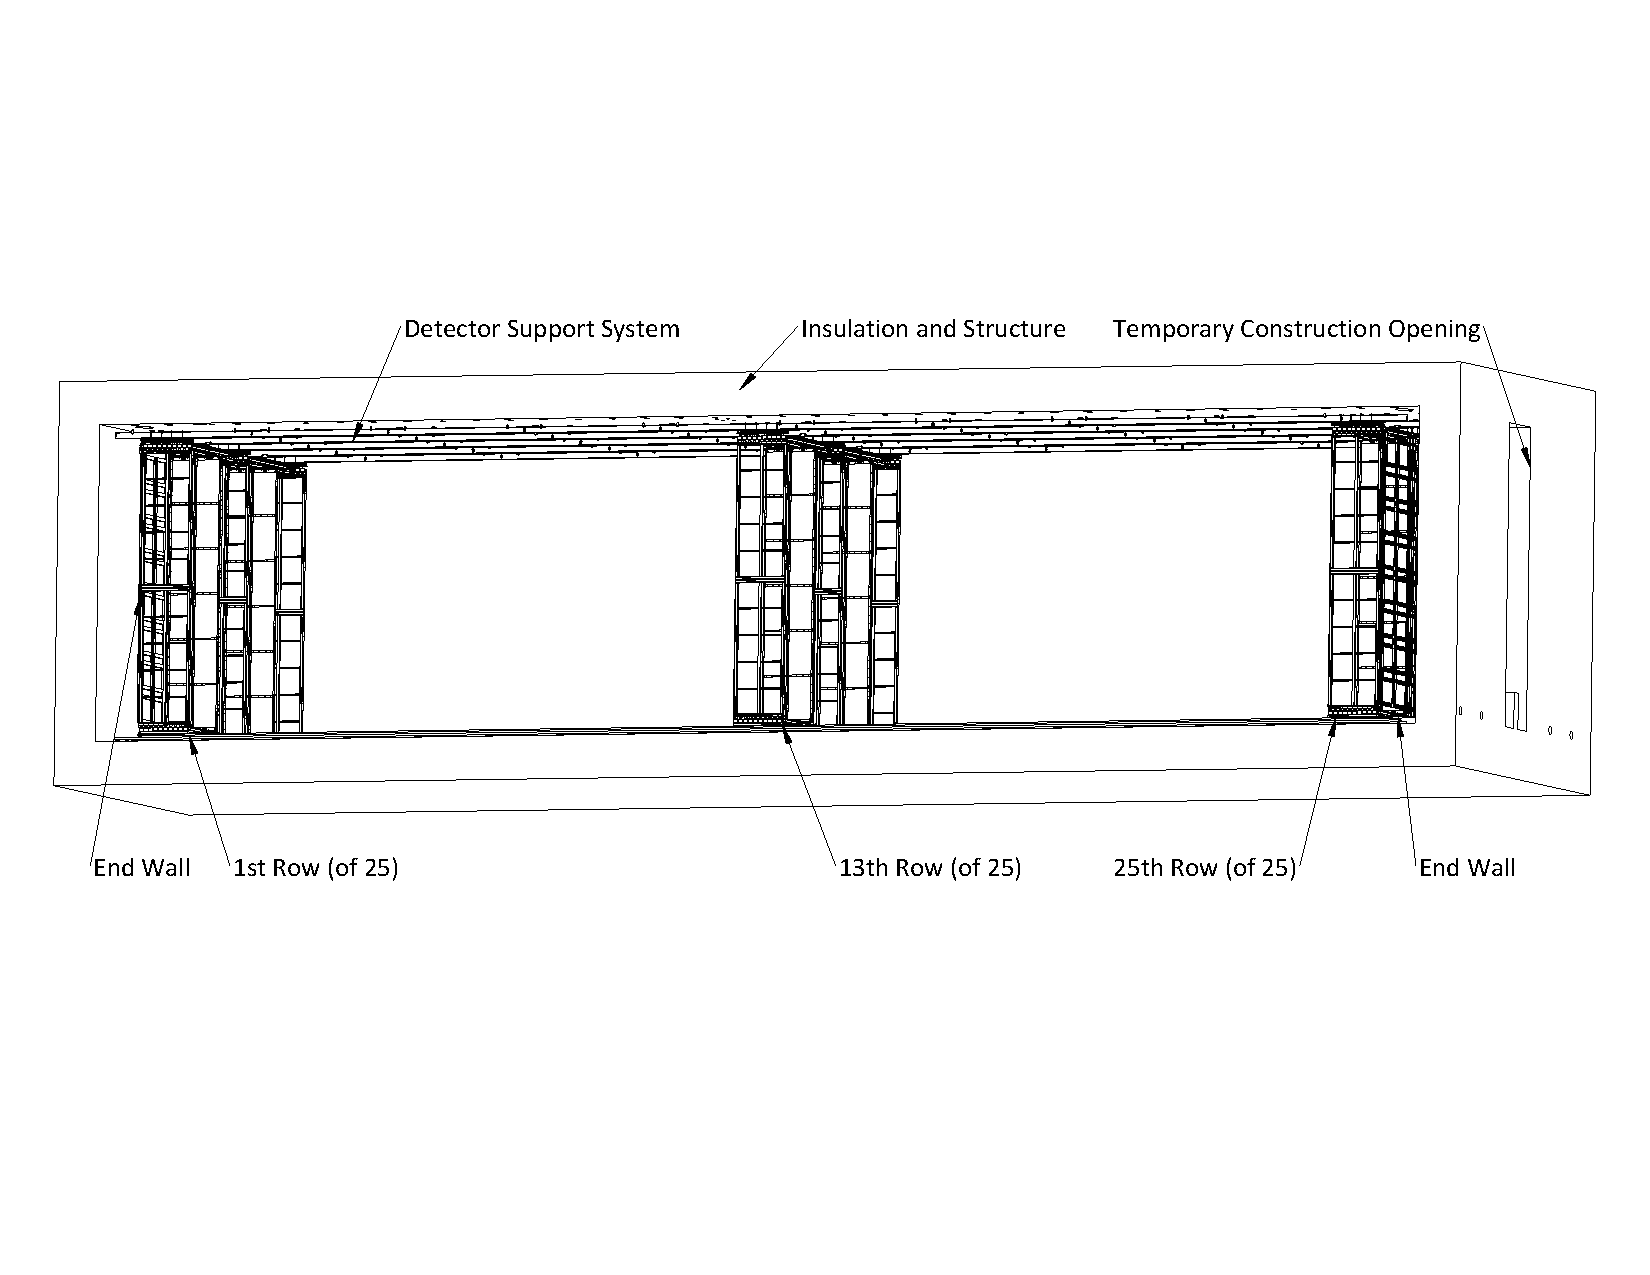
\includegraphics[width=0.85\textwidth]{Overall_model_SP}
\end{dunefigure}
As mentioned earlier, this model does not include all the details of
the detector components. The components are simplified to keep the
overall model complexity to a manageable level.


Figure~\ref{fig:dune-sp_row} shows the model of one row of the
detector module. Each row is constructed from six \dwords{apa}, four
\dwords{cpa} and eight \dwords{fc} and \dwords{gp}. A total of 25 rows
comprise one \dword{dsp} far detector.
\begin{dunefigure}[Model of one row of \dword{dsp}]{fig:dune-sp_row}
  {Model of one row of \dword{dsp} module showing overall arrangement and dimensions.}
  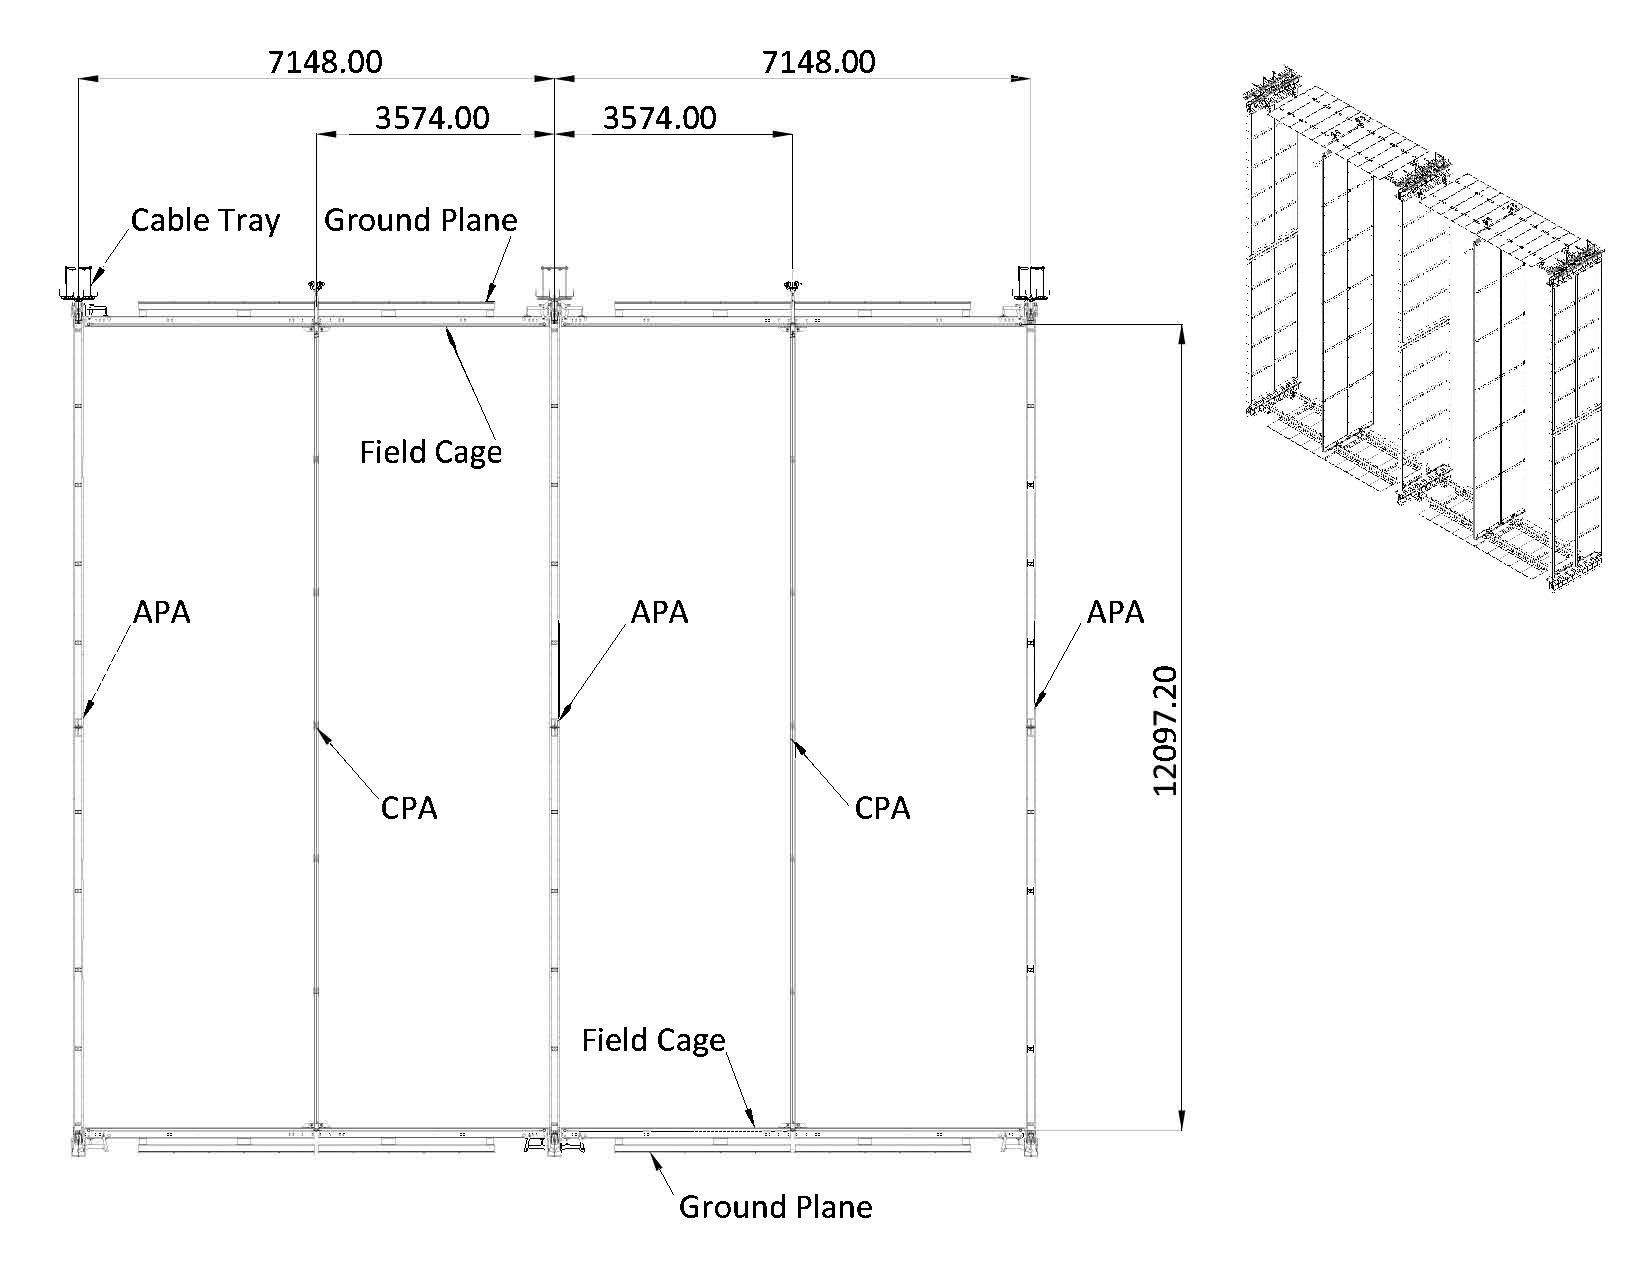
\includegraphics[width=0.85\textwidth]{Model_one_row_SP.pdf}
\end{dunefigure}


Figure~\ref{fig:dune-sp_transverse} shows a cross section of the
\dword{dsp} far detector in the transverse direction and the overall
dimensions.
\begin{dunefigure}[Section view of the \dword{dsp} in the
    transverse direction]{fig:dune-sp_transverse}
  {Section view of the \dword{dsp} in the transverse
    direction.}
  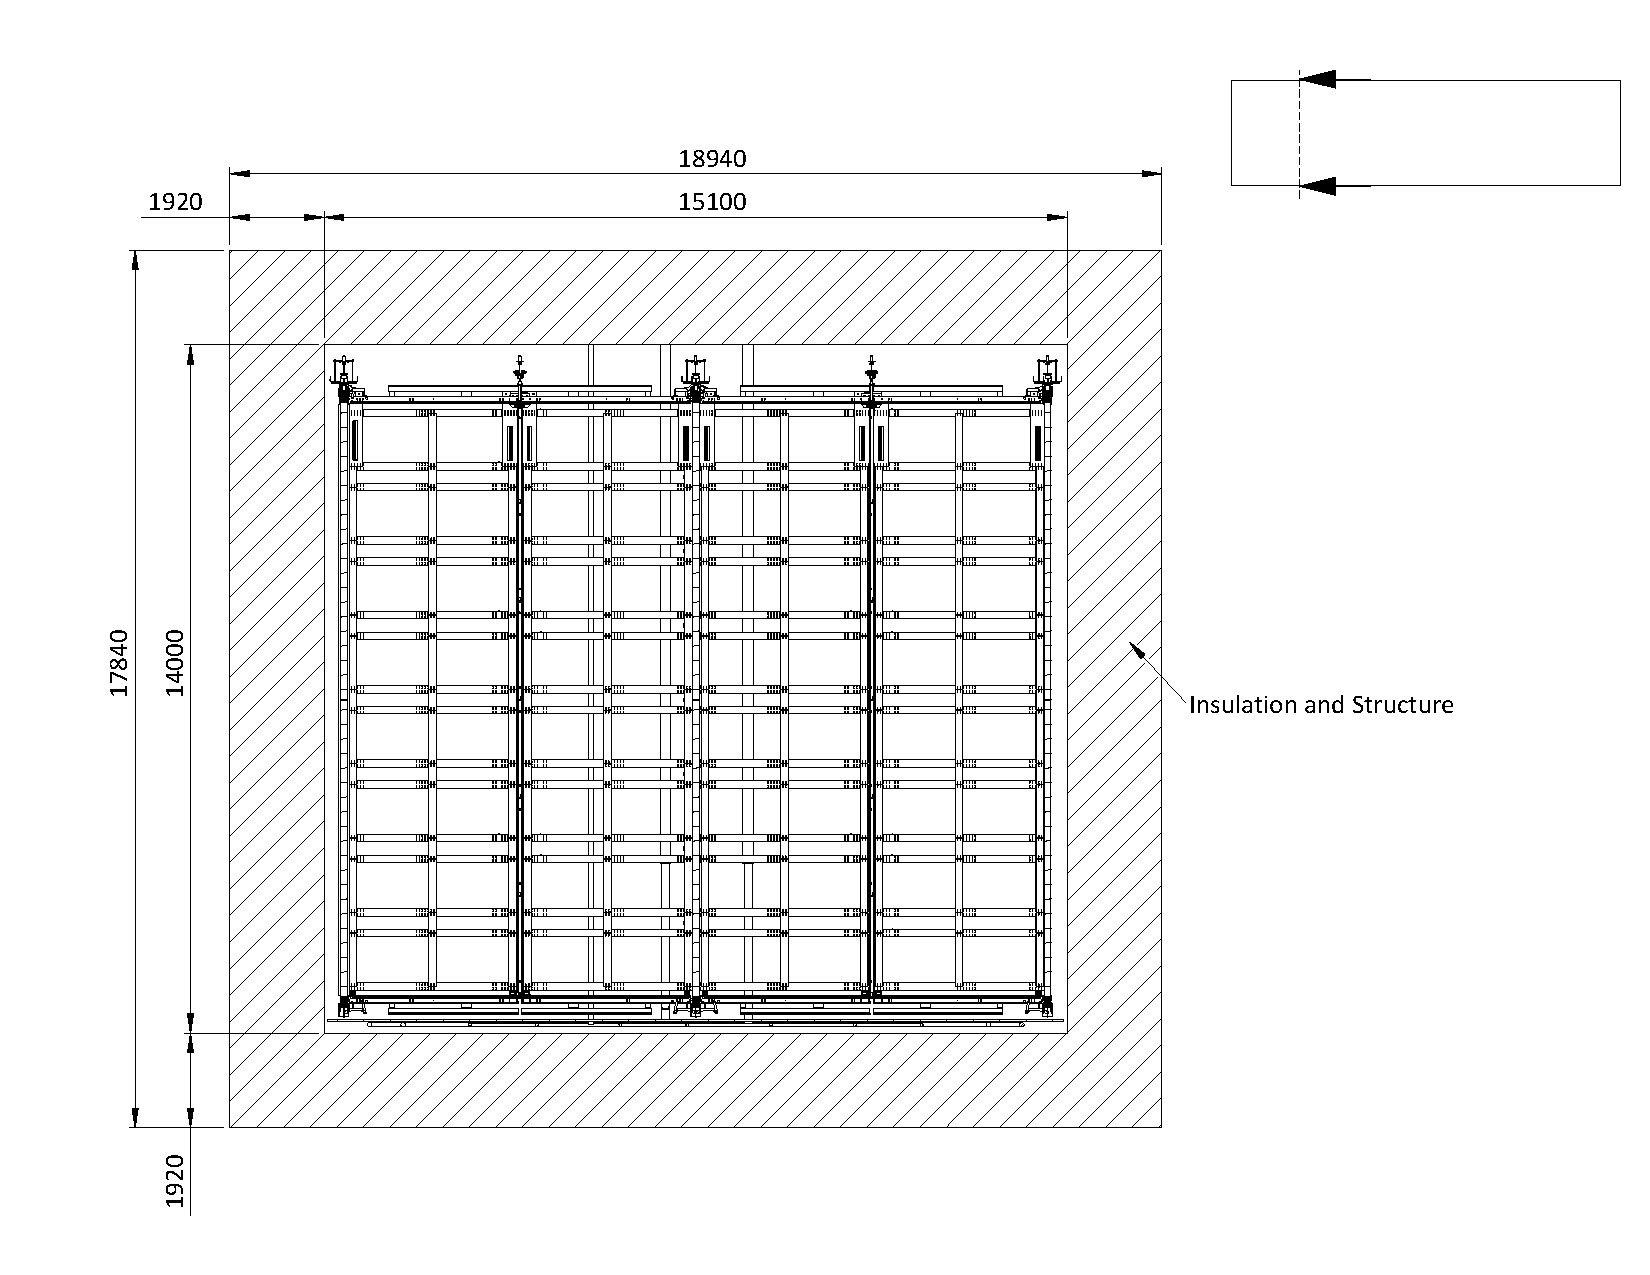
\includegraphics[width=0.65\textwidth]{SP_transverse_section.pdf}
\end{dunefigure}
Figure~\ref{fig:dune-sp_long} shows a cross section of the
\dword{dsp} far detector in the longitudinal direction and the overall
dimensions.In both figures, the cryostat structure and insulation are shown
as cross-hatched areas.
\begin{dunefigure}[Overall model of the \dword{dsp} in the
    longitudinal direction]{fig:dune-sp_long}
  {Overall model of the \dword{dsp} module in the longitudinal direction.}
  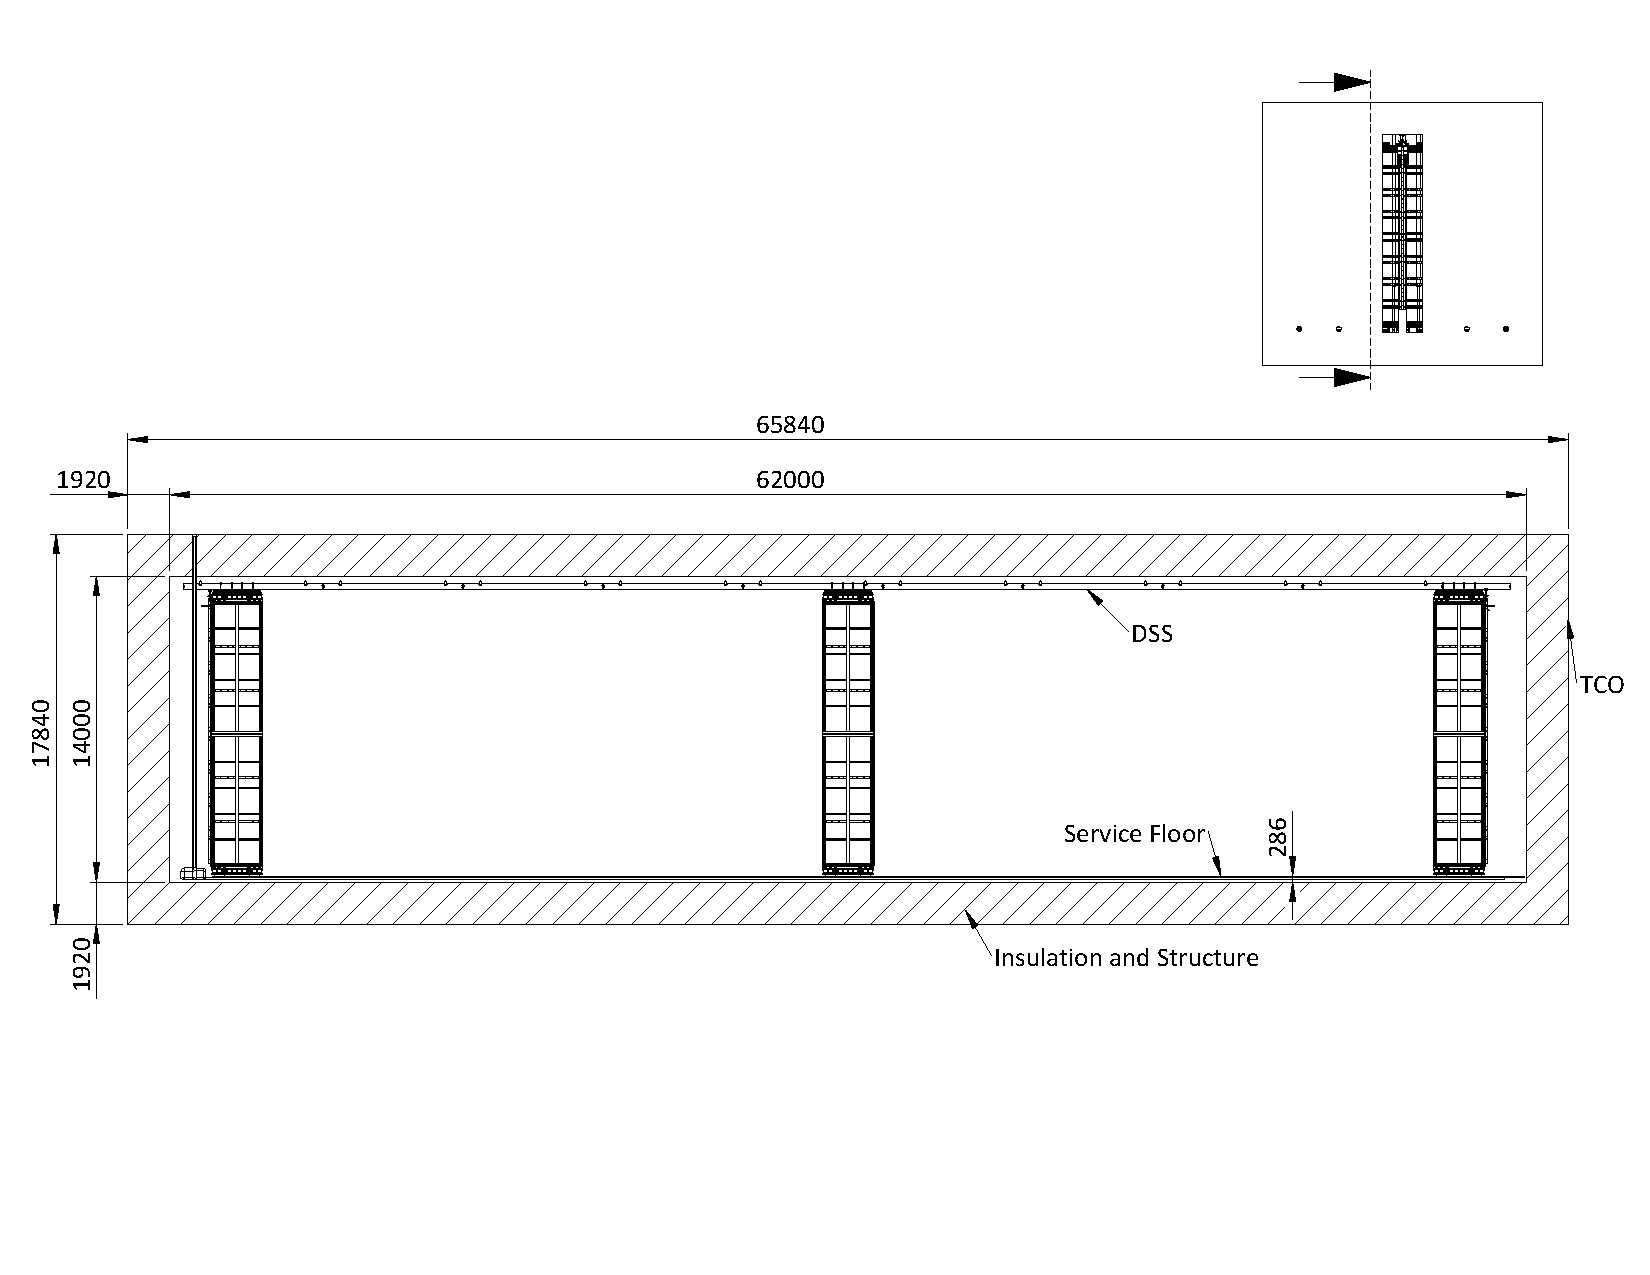
\includegraphics[width=0.85\textwidth]{SP_longitudinal_section.pdf}
\end{dunefigure}



Figure~\ref{fig:dune-dp_overall} shows the overall model of the dual
phase detector, \dword{ddp}. One wall of the cryostat is removed to
show the interior components. The detector has 20 rows, all of which
are constructed the same. Each row comprises four \dwords{crp},
cathode, \dword{gp}, \dwords{pmt} and side-wall \dwords{fc}.  At the
end of row one and row 20, end walls are installed which close the
detection volume.
\begin{dunefigure}[Overall model of the \dword{ddp} modeul]{fig:dune-dp_overall}
  {Overall model of \dword{ddp} module.}
  \fbox{\parbox[c][6cm]{6cm}{
      \begin{center}
        Dummy Dual-phase figure
      \end{center}
  }}
  %  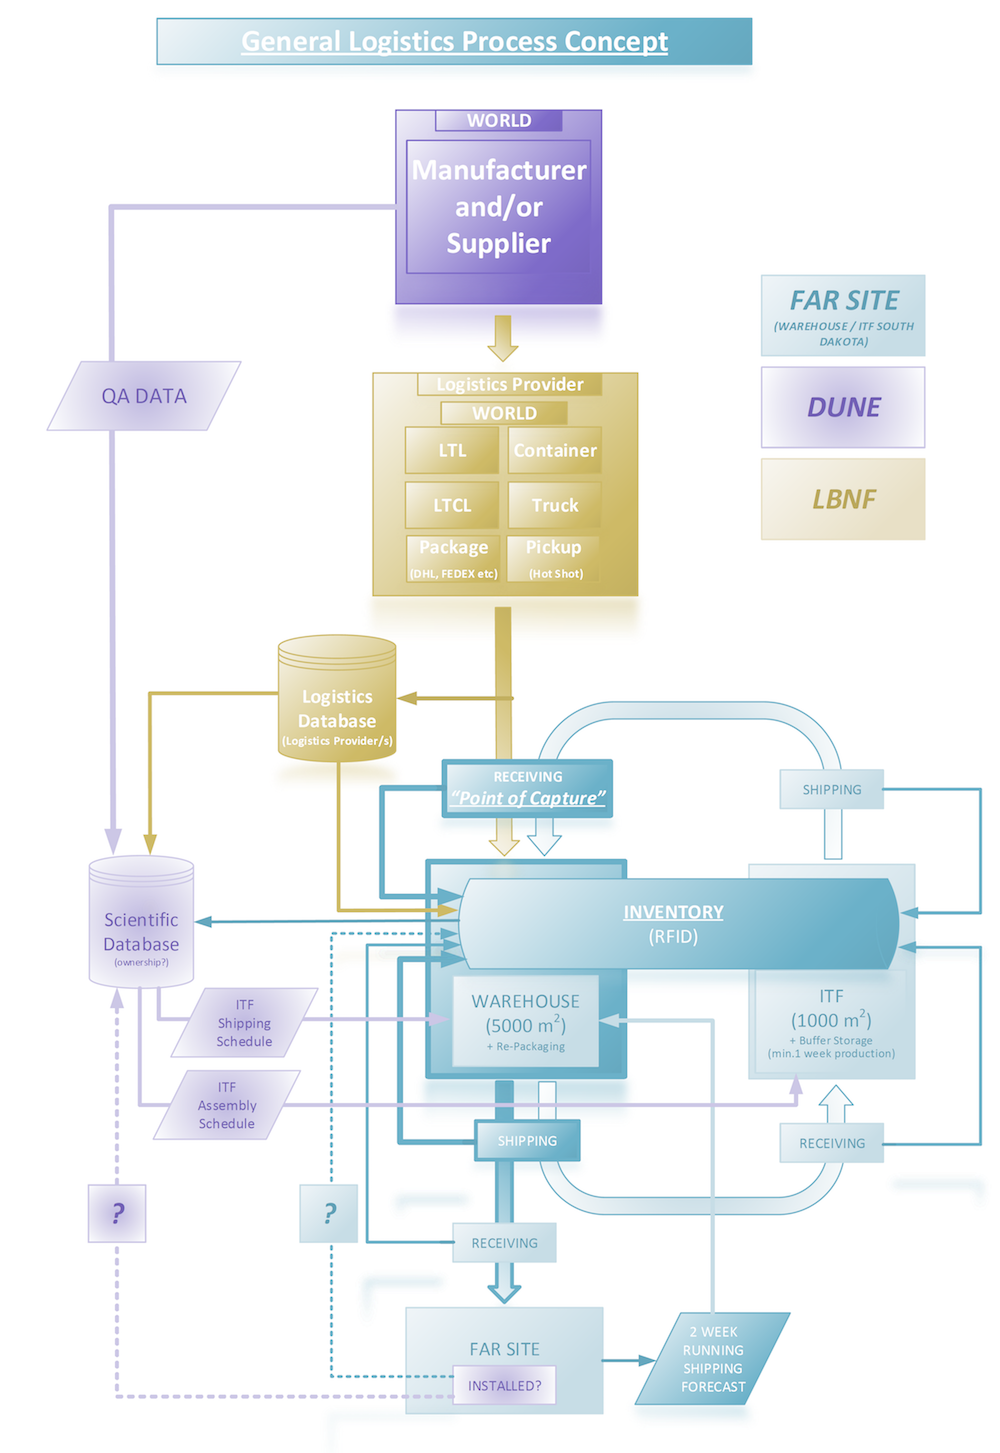
\includegraphics[width=0.85\textwidth]{logistics}
\end{dunefigure}


More detailed models of the \dword{ddp} detector integration
interfaces are shown in the following figures.
\fixme{Need analogous figures and explanations for Dual Phase}

\subsection{Envelope and Assembly Models}
\label{sec:fdsp-coord-integ-envelope}

Static models represent the detector and its components using their exact
design dimensions. Such exact dimensions are needed so the
detail component drawings and model are completely compatible at all
times.


For installation and operation, however, other envelope models are
needed. Envelope models are developed to address issues that affect
installation and operation:
\begin{enumerate}
 \item Effects on the detector caused by distortion of the cryostat
   and detector support structure due to gravity
 \item Effects on the detector caused by distortion of the cryostat
   and detector support structure due to loads on the cryostat during
   detector filling and operation
 \item Effects on the detector caused by thermal contraction during
   detector filling and operation
 \item Effects of component and
   assembly tolerances
 \item Clearances needed for installation and envelopes needed for
   access and tooling
 \item Reference models and drawings needed for installation stages
   and to control assembly
 \item Reference models and drawings needed for alignment and survey
\end{enumerate}


The models and drawings described above are generated from static
models. Models are also generated to represent combined effects of the
above. In all cases, as with static models, 2D drawings are created
and provide the basis for the installation drawings.


Generating envelope models and drawings are the responsibility of the
\dword{tc} engineering team in coordination with consortia.


\subsection{Integration and Interface Drawings}
\label{sec:fdsp-coord-integ-drawings}

Within each detector, components from various consortia are assembled
and installed. In addition, components that are the responsibility of
\dword{tc} are also assembled and installed in parallel. The interfaces
among components are developed and managed through models and drawings
as described in Section~\ref{sec:fdsp-coord-integ-models}. Many such
interfaces must be controlled. The following section shows some of the
interfaces, controlling drawing, dimensions, and configurations.


Figure~\ref{fig:dune-apa_interfaces_top} shows the interfaces for the
top \dwords{apa} in the upper corner of the cryostat. It also shows the position
of the cable penetration for the \dword{apa}. Interfaces with cryostat
corrugations and \dword{lar} fill lines are also shown. The reference plane,
which is defined as the plane of the \dword{apa} yokes is explained in the
alignment section.
\begin{dunefigure}[Interface between upper \dword{apa},
    \dword{fc}, cable trays and \dword{dss}]{fig:dune-apa_interfaces_top}
  {\dword{dsp} interface between upper \dword{apa}, \dword{fc}, cable
    trays and \dword{dss}.}
  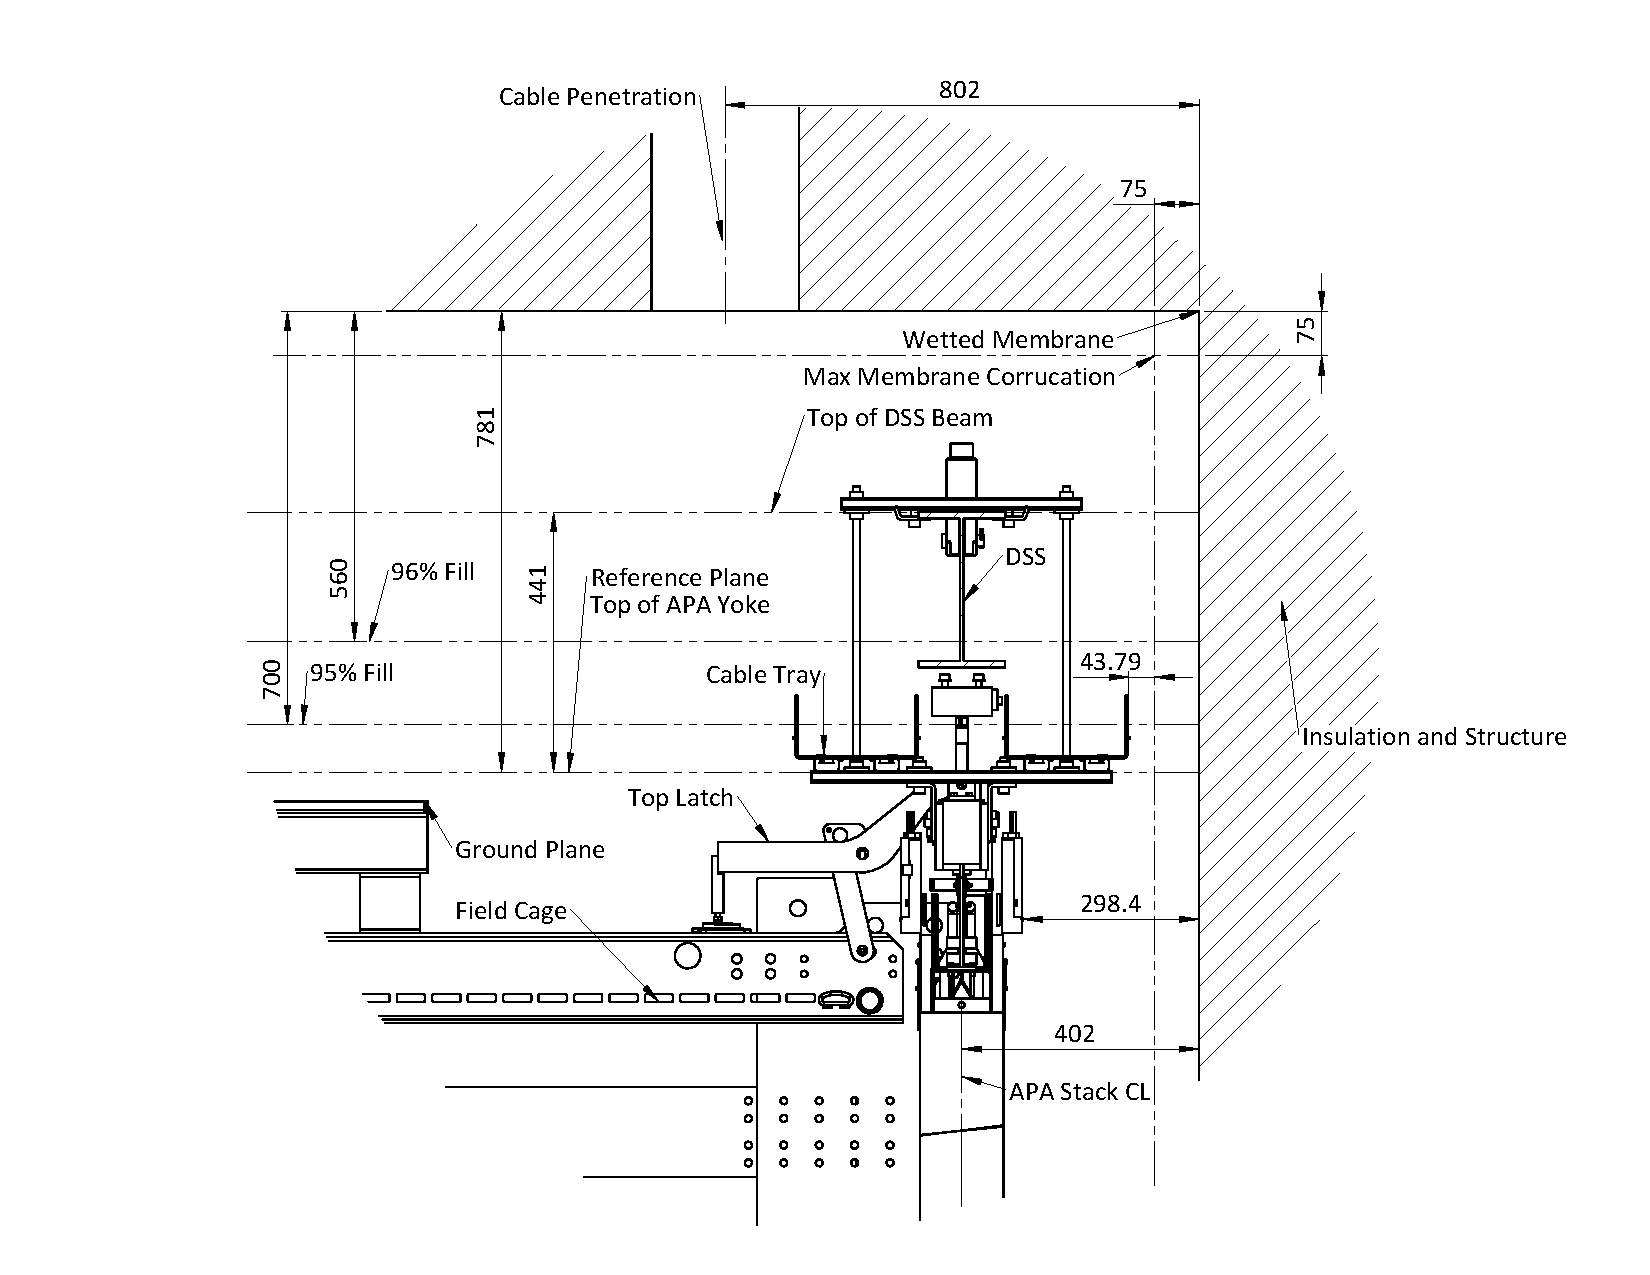
\includegraphics[width=0.8\textwidth]{Interface_upper_apa.pdf}
\end{dunefigure}


Figure~\ref{fig:dune-apa_interfaces_bottom} shows the interfaces for
the bottom \dwords{apa} in the lower corner of the cryostat. In both figures,
the connection latch between the \dwords{fc} and \dwords{apa} is also
shown.
\begin{dunefigure}[Interface between lower \dword{apa}, \dword{fc}
    and service floor]{fig:dune-apa_interfaces_bottom}
  {\dword{dsp} interface between lower \dword{apa}, \dword{fc} and 
    service floor.}
  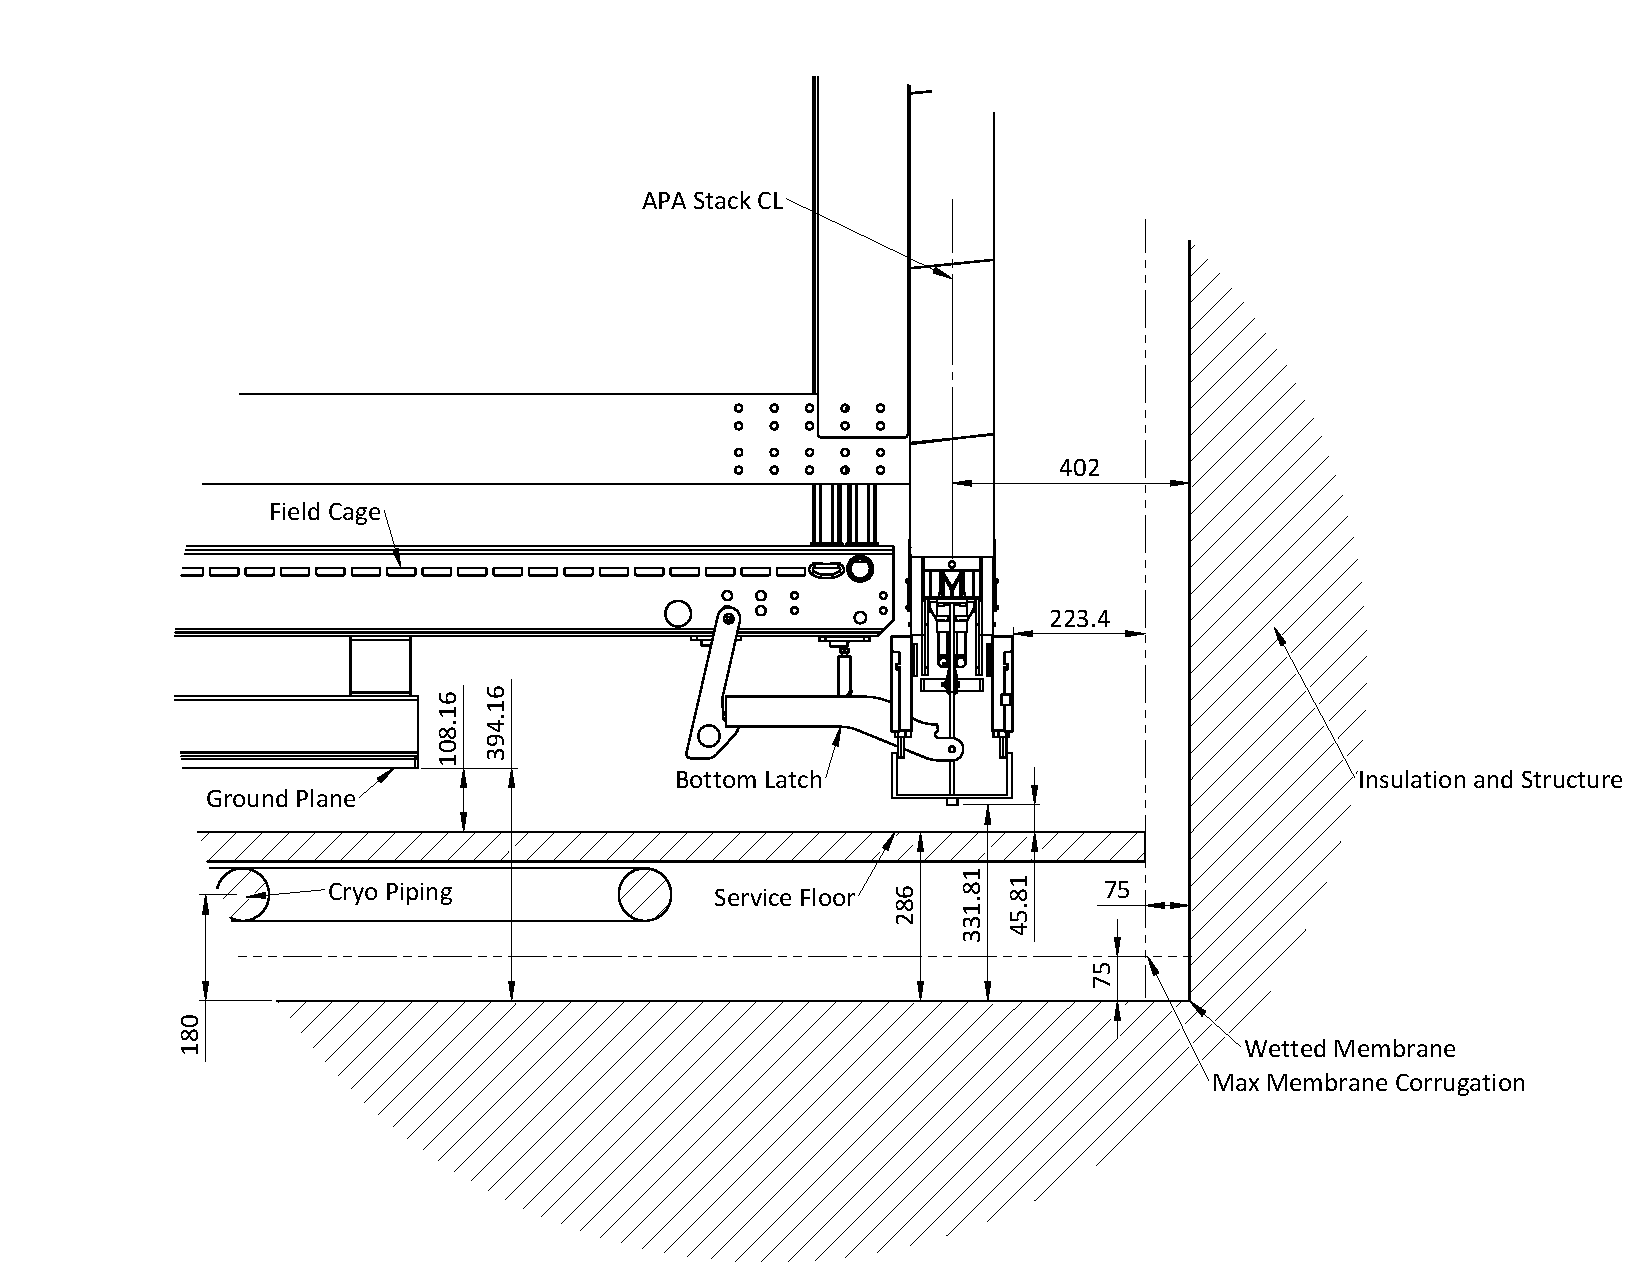
\includegraphics[width=0.7\textwidth]{Interface_lower_apa.pdf}
\end{dunefigure}


Figure~\ref{fig:dune-apa_interfaces_mid} shows the interfaces for the
top of the central row of \dwords{apa} with other components. In this case, a
double latch connection is used. Similarly,
Fig~\ref{fig:dune-cpa_interfaces} shows the interfaces for top of the
\dwords{cpa} with other components.
\begin{dunefigure}[Interface between \dword{apa}, upper \dword{fc} 
    and \dword{gp}]{fig:dune-apa_interfaces_mid}
  {\dword{dsp} interface between \dword{apa}, upper \dword{fc} and \dword{gp}}
  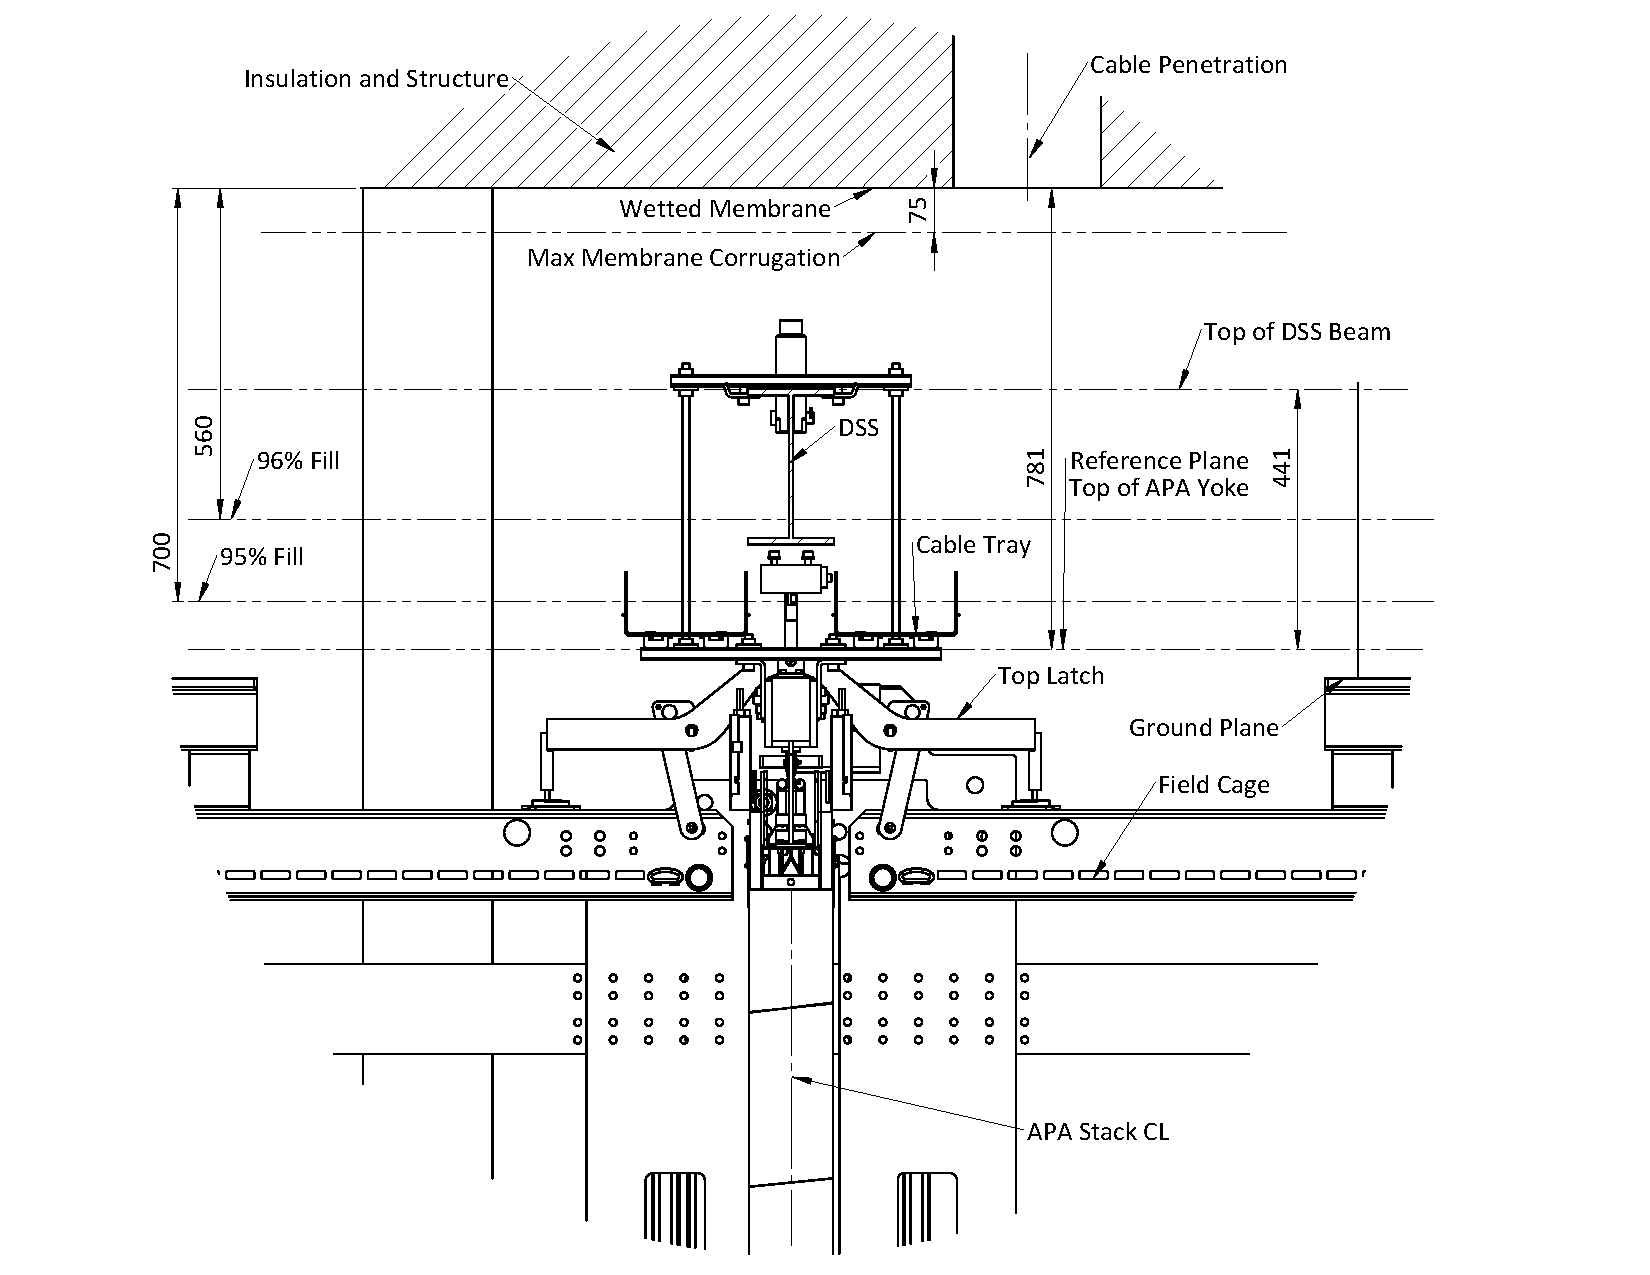
\includegraphics[width=0.8\textwidth]{Interface_upper_mid_apa.pdf}
\end{dunefigure}
\begin{dunefigure}[Interface between \dword{cpa}, upper \dword{fc} and \dword{gp}]
    {fig:dune-cpa_interfaces}
  {\dword{dsp} interface between \dword{cpa}, upper \dword{fc} and \dword{gp}.}
  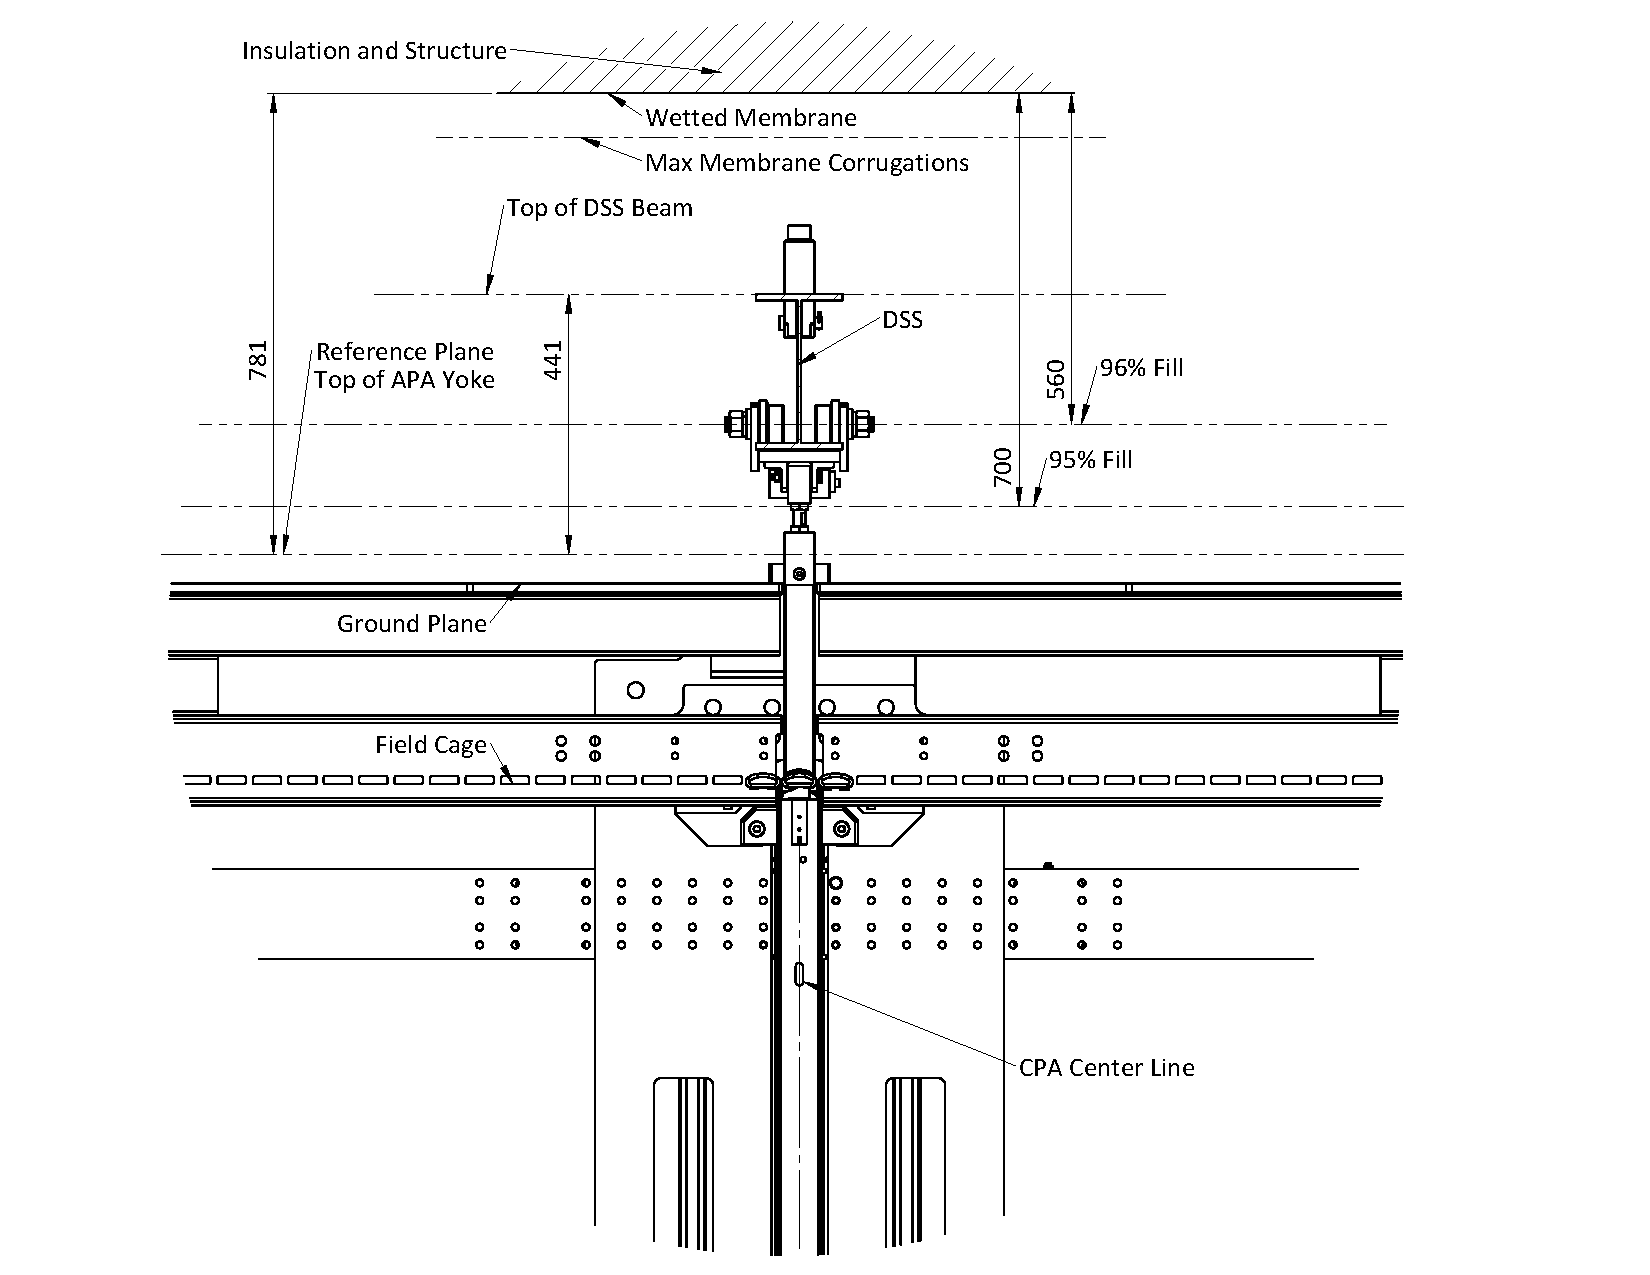
\includegraphics[width=0.8\textwidth]{Interface_upper_cpa.pdf}
\end{dunefigure}

These integration drawings are derived directly from the overall
integration model. The overall integration model is assembled from
component models developed by the consortia. Interfaces are controlled
by \dword{tc} and consortia maintain their model files to be
compatible with the interfaces. During the design phase, models are
assembled and checked continuously. At the time of final design, all
interfaces will be fixed.


Component tolerances and installation clearances are managed through
additional models as described in
Section~\ref{sec:fdsp-coord-integ-envelope}.
Fig~\ref{fig:dune-apa_envelope} shows the \dwords{apa} and
\dwords{cpa} as well as their relative positions that show how they are
constrained within the detector.
\begin{dunefigure}[Graphical representation of envelope dimensions and
    installation clearances for \dwords{apa} and \dwords{cpa}
    in the warm state]{fig:dune-apa_envelope} {\dword{dsp} graphical
    representation of envelope dimensions and installation clearances
    for \dwords{apa} and \dwords{cpa} in the warm state.}
  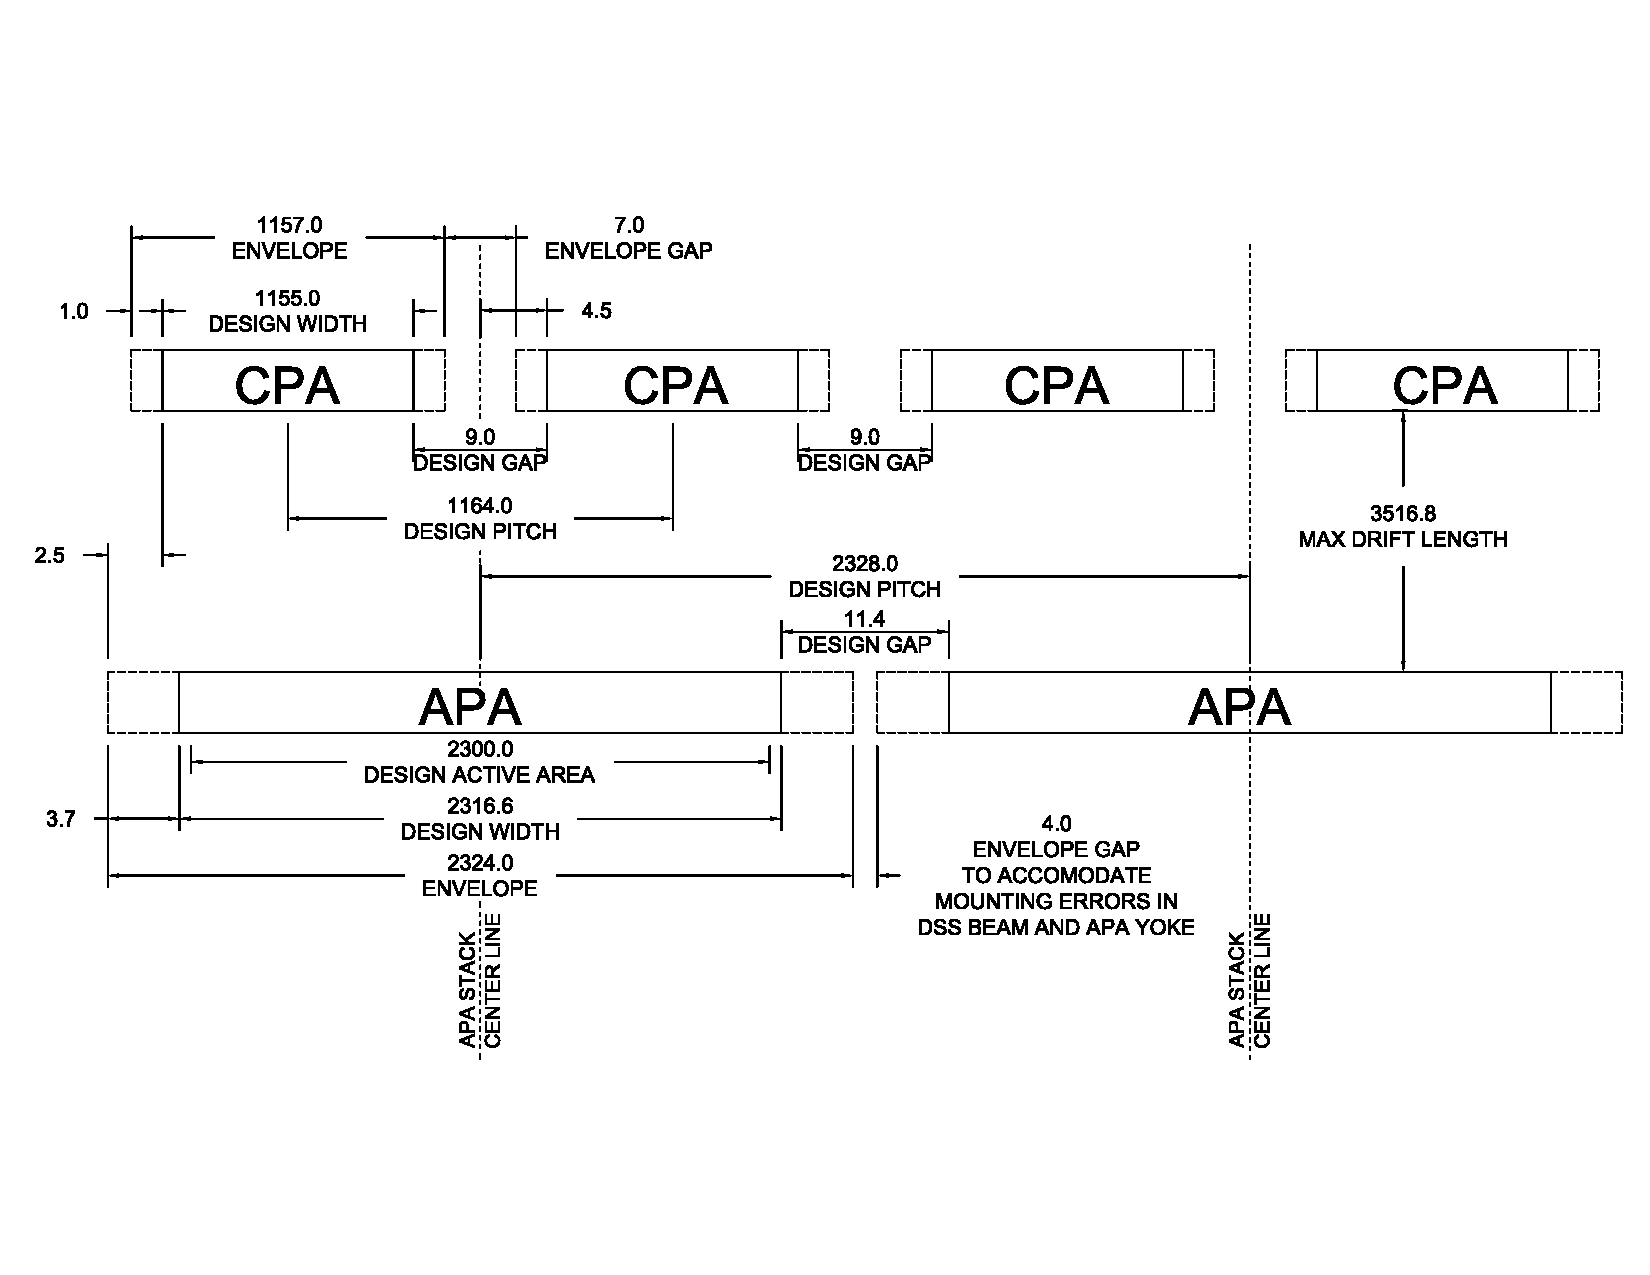
\includegraphics[width=0.95\textwidth]{Warm_envelope_dimensions.pdf}
\end{dunefigure}


This figure shows design dimensions. Component tolerances and assembly
tolerances for the upper and lower \dwords{apa} and \dword{cpa} stacks
have been analyzed and represented as envelope dimensions. An envelope
gap has been defined to account for tolerances in the support system
position and among components. Taking all of these into account, pitch
distances for \dwords{apa} and \dwords{cpa} have been defined in the
warm state.

Figure~\ref{fig:dune-apa_envelope} also shows the design drift distance in
the warm state. The drift distance is defined as the perpendicular
distance between the surface of \dwords{cpa} and the collection wire
plane of \dwords{apa}.

\Dwords{apa} and \dwords{cpa} are supported in groups of two or three
on \dword{dss} beams. There are 50 beams arranged into five parallel
rows with 10 beams in each row.  In the cold state, the relative
positions between groups of \dwords{apa} which are supported on
different beams change due to thermal contraction of the
beams. Relative positions within each group which are supported on the
same beam are relatively constant because \dwords{apa} and
\dword{dss} are made from stainless steel.  The effect is that the gap
in the active area between some \dwords{apa} increases.  As can be
seen in Figure~\ref{fig:dune-apa_aa_cold} in the warm state, the gap
in the active areas between adjacent \dwords{apa} is 28 mm (dotted
line). In the cold state, nine of the 24 gaps increase to
approximately 45 mm.
\begin{dunefigure}[\Dwords{apa} active area gap in cold state]{fig:dune-apa_aa_cold} 
    {\dword{dsp} gap in active areas between adjacent \Dwords{apa} in the cold state. Dashed line warm sate, dots cold state.}
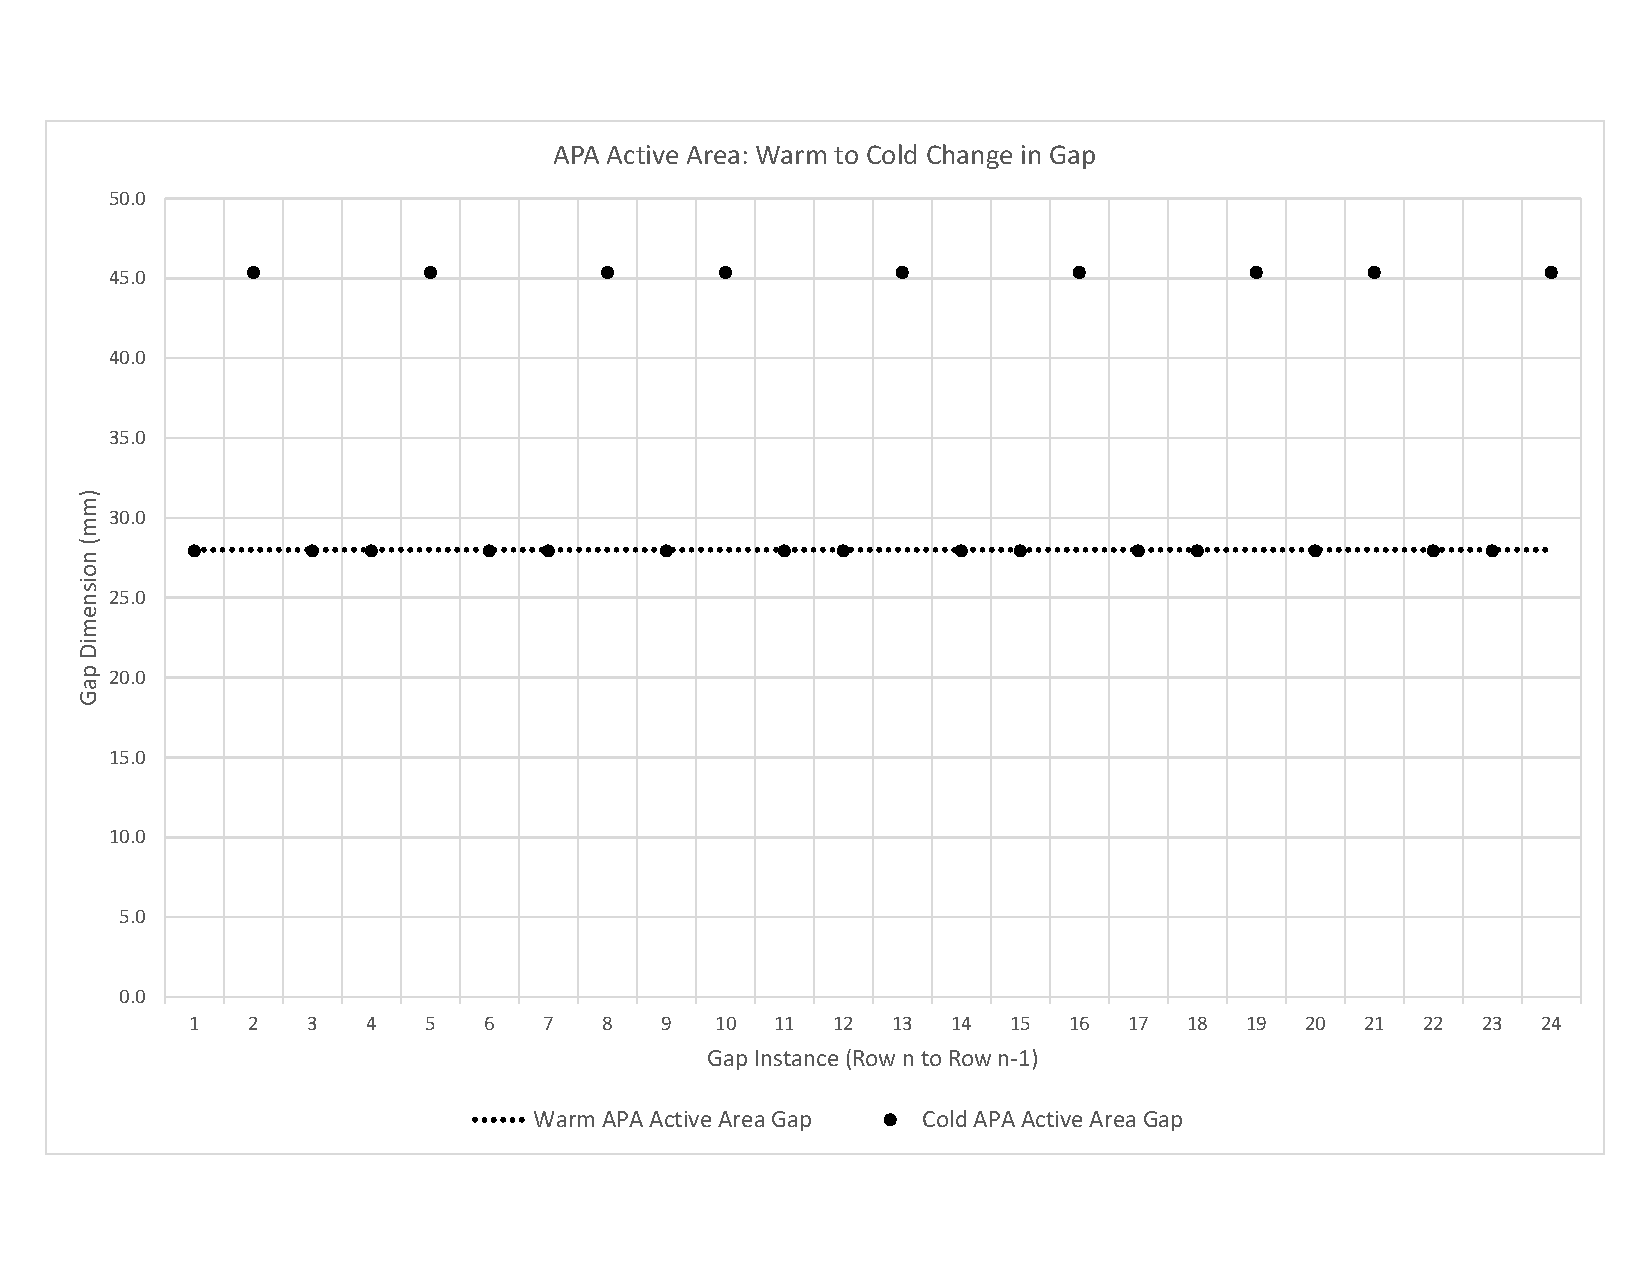
\includegraphics[width=0.8\textwidth]{apa_aa_gap_change.pdf}
\end{dunefigure}

The effects of gravity and buoyancy are not represented in above
analysis. Such effects are under study and will be shown in the models
as design progresses.


Before installing the detector, a set of cryogenic distribution pipes
are installed on the floor of the cryostat. In addition, the membrane
of the cryostat will have corrugations that impede
movement. Therefore, a temporary service floor will be installed. The
floor will be installed, and later removed, in
sections. Figure~\ref{fig:dune-floorpipes} shows the interface of the
service floor with other components.
\begin{dunefigure}[\dword{dsp} interface of cryogenics, service floor and detector]{fig:dune-floorpipes} 
{\dword{dsp} interface of cryogenic distribution pipes, service floor, and
  detector.}
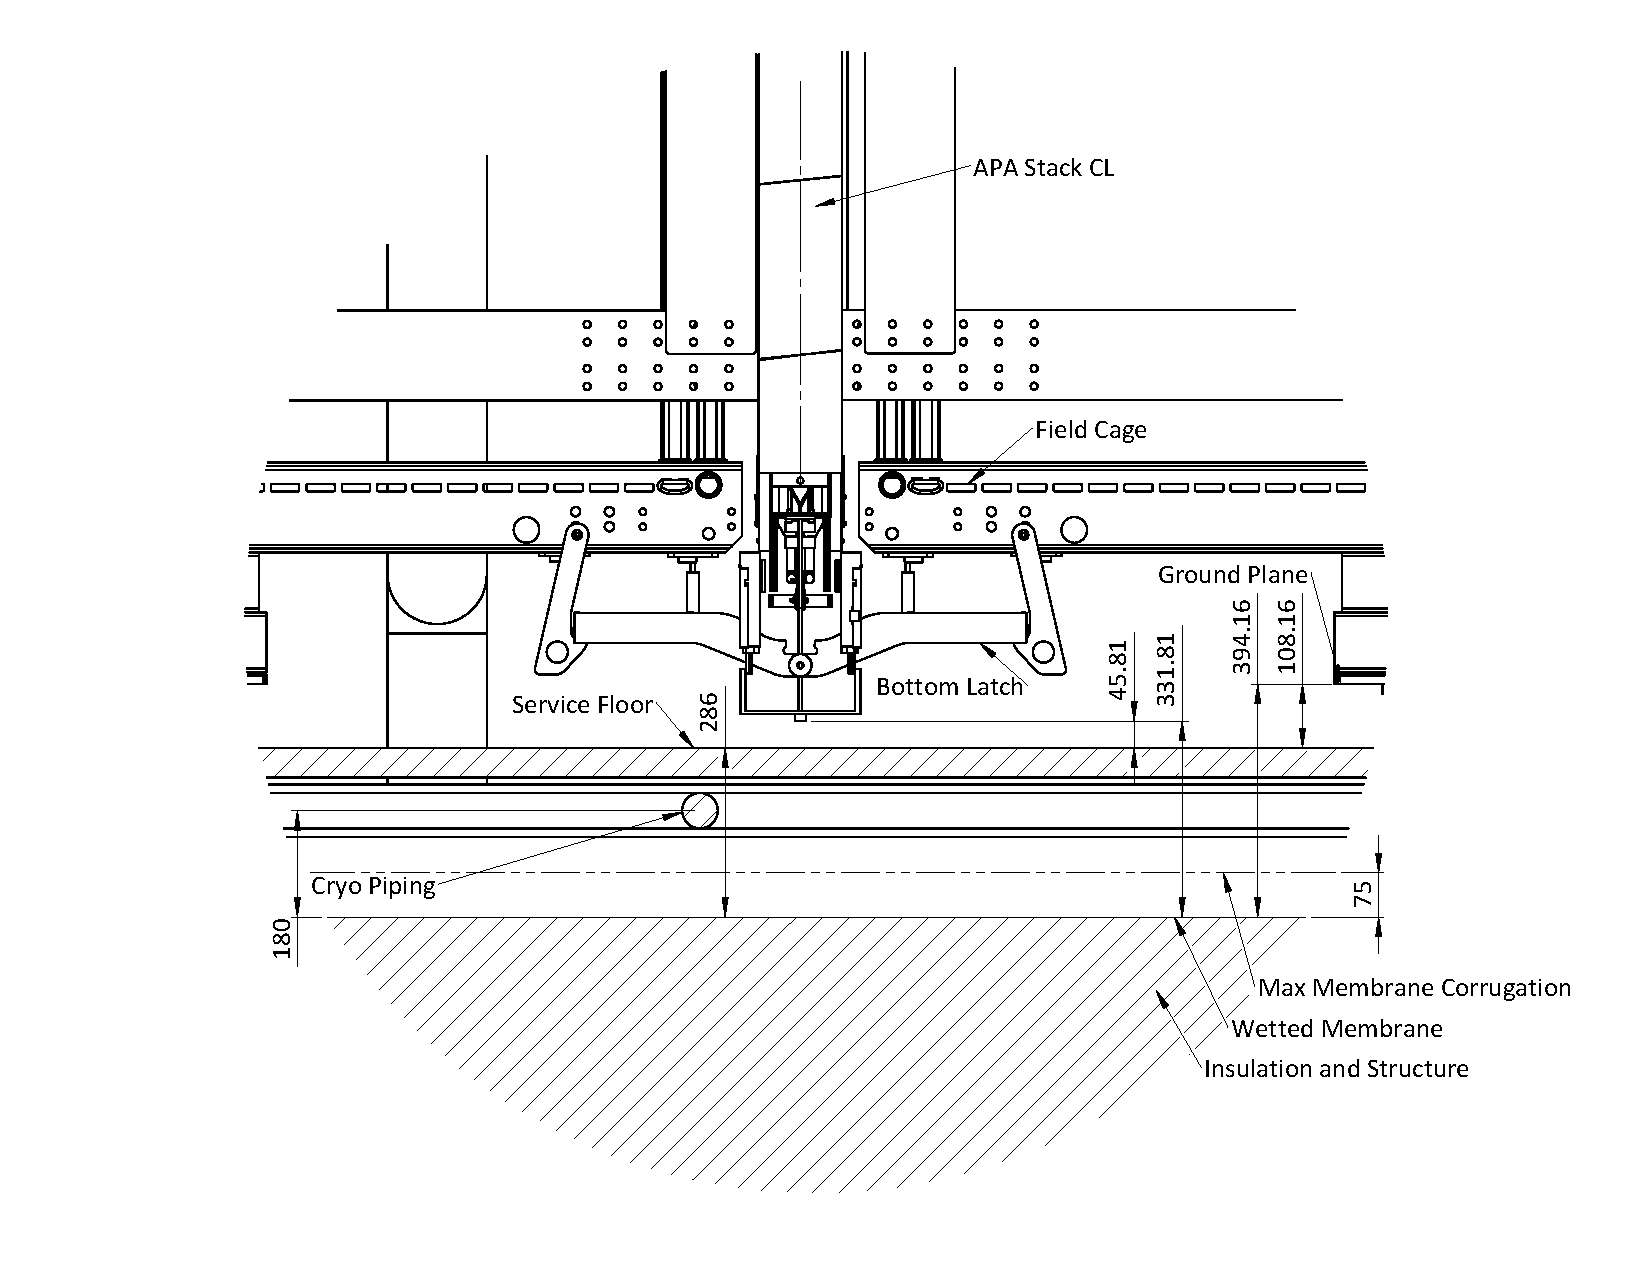
\includegraphics[width=0.8\textwidth]{Interface_lower_mid_apa.pdf}
\end{dunefigure}
\fixme{Need analogous figures and explanation for Dual Phase}

\subsection{Detector Survey and Alignment}
\label{sec:fdsp-coord-integ-survey}
The detector placement within the cryostat inside the
cavern does not have a physics requirement. The requirement is driven
by overall mechanical assembly needs so that interfacing
parts are assembled properly and function as intended.


In this section, reference frames for the detector are defined so the
overall survey and alignment can be done within the cavern reference
frame. (Note: we have not yet defined this.)


For the single-phase detector, a flat and level reference plane is
defined that is coplanar with the upper \dword{apa} yoke planes. Thus,
75 yoke planes define this flat and level reference plane. This
reference plane is set at exactly 781 mm below the theoretical plane
of the cryostat top membrane.


The detector reference plane is coplanar with the upper \dword{apa}
yoke planes because all features, including the active area, are
referenced to this plane.  Once this reference plane is defined and
established through survey, all vertical distances within the detector
are referenced and established relative to this plane.
Figure~\ref{fig:dune-apa_interfaces_mid} shows the reference plane in
relation to the cryostat top membrane and \dword{dss}.


During installation, the height of the \dword{dss} beams is set in
accordance with this relationship. Adjustments are made in the
\dword{dss} to ensure all the beams are in the correct plane. The
combined effects of gravity, buoyancy, temperature and LAr mass after
fill are calculated, and further adjustments are made to
compensate. This will ensure that the detector is as close as possible
to design value after fill.


The transverse position of the detector is constrained to the center
of the cryostat. Thus, the mid-plane of the middle row \dword{apa} is
coplanar with the vertical mid-plane of the cryostat. This
relationship is verified when the \dword{dss} beams and central row of
\dwords{apa} are installed. The outer rows are similarly aligned and
surveyed with the offset as shown in Figure~\ref{fig:dune-sp_row}.
\begin{dunefigure}[Position of longitudinal
    reference point for \dword{dsp}]{fig:dss_feedthru}
  {Position of feedthrough determining the longitudinal reference point of the \dword{dsp} module.}
  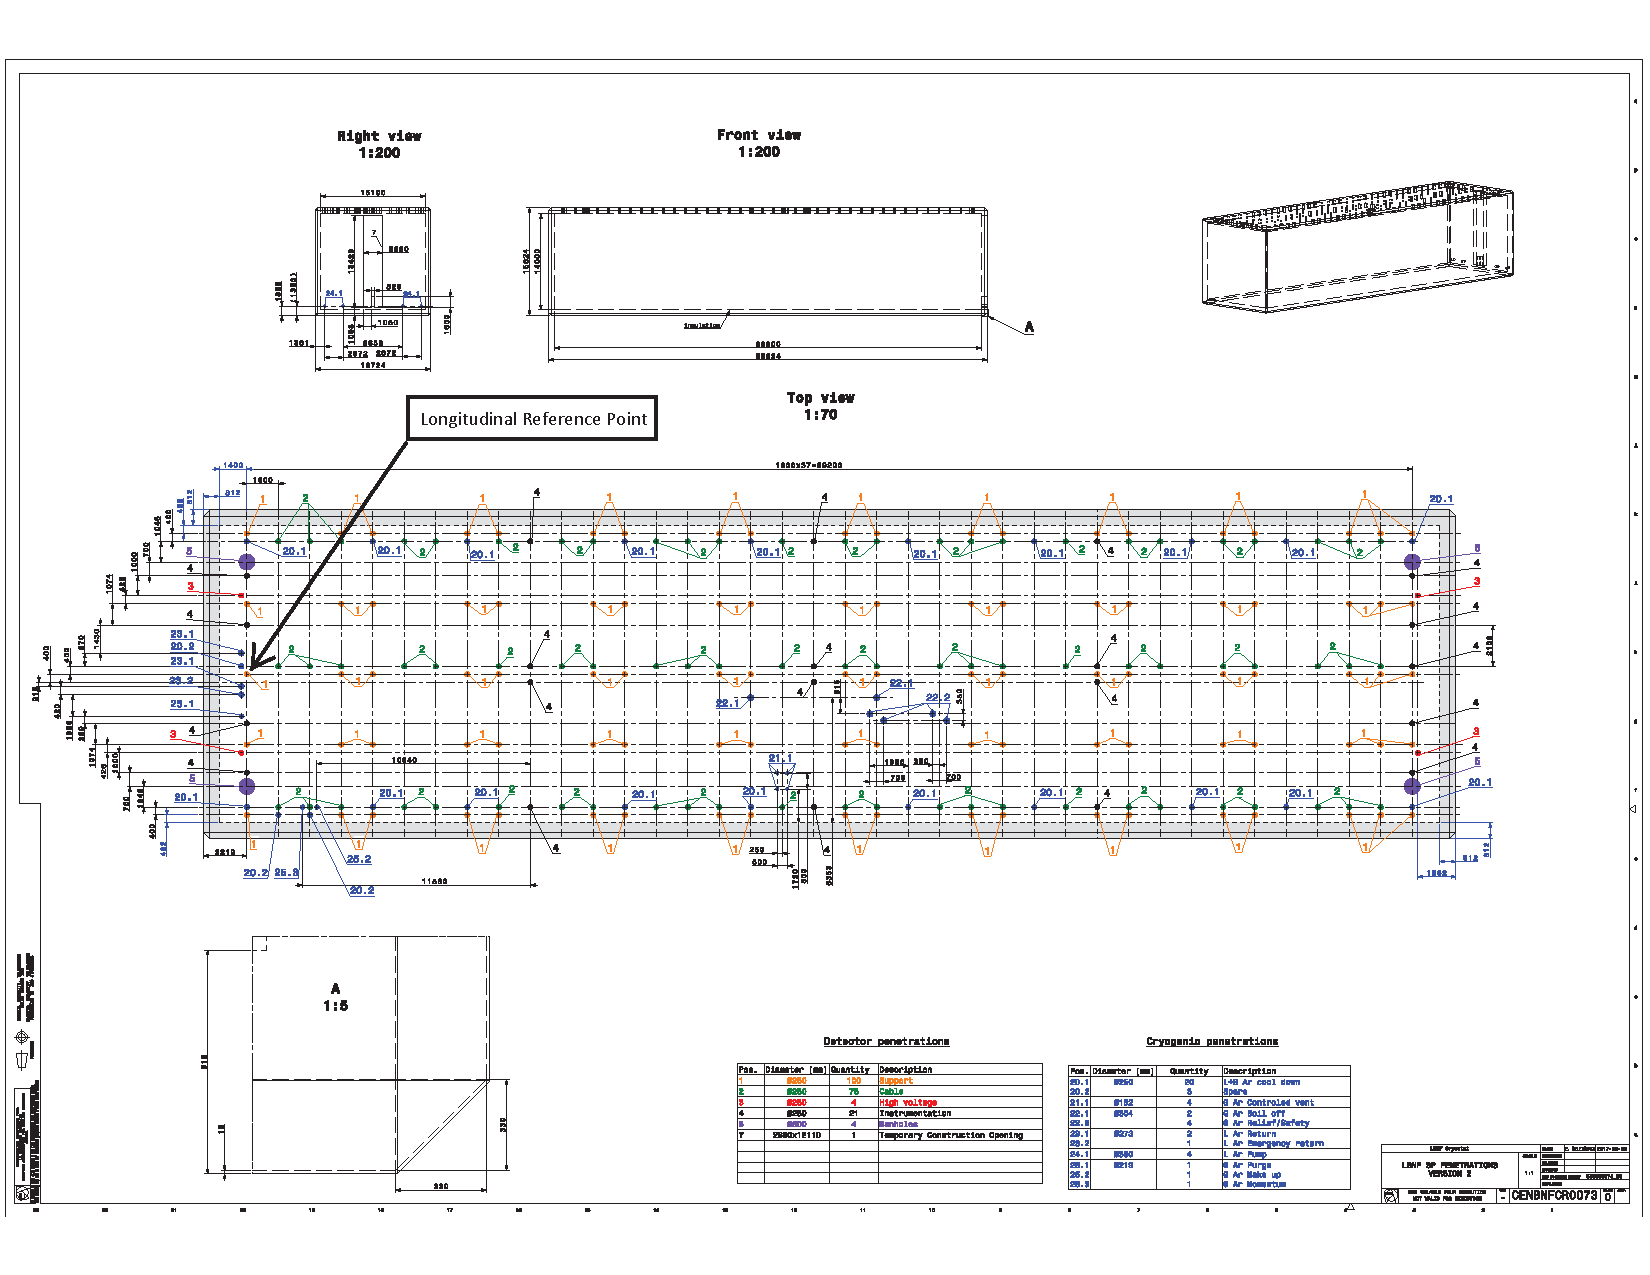
\includegraphics[width=0.9\textwidth]{SP_longitudinal_reference.pdf}
\end{dunefigure}


The longitudinal reference point of the detector within the cryostat
is defined by the position of the single feedthrough of the central row
farthest from the cryostat opening. This feedthrough position
is shown in Figure~\ref{fig:dss_feedthru}.


\fixme{NOTE TO TC: Dual phase should be similar transversely and
longitudinally, vertically, it needs to be determined}




\section{Electrical Integration}
\label{sec:fdsp-Integ-electrical}



\subsection{Electrical System Block Drawings, Schematics, Layouts and Wiring Diagrams}
\label{sec:fdsp-coord-electrical}


\dword{tc} is responsible for the AC power
distribution supplied to the experiment and to detector electronics
racks.  This is described in section~\ref{sec:fdsp-coord-faci-grounding} 
and section~\ref{sec:fdsp-coord-faci-power}.  Specific guidance has been provided
regarding the use of DC power supplies and cable shield treatment.
These guidelines are specified in EDMS-2095958.  They are the same as
were followed at \dword{protodune} and developed during extensive testing of
the APA wire readout at BNL and \dword{protodune}.  Guidelines are included
for the treatment of DC power supplies and the use and connection of
shielded cables.  All systems are reviewed for compliance to these
guidelines during the design review procedure.  Any deviation from the
guidelines must be noted and approved by system engineering.

\dword{tc} will, through the design review process, insure
that all electrical systems are following safe design practice and
will pass operational readiness reviews.  Operational Readiness
Reviews will fall under the Authority Having Jurisdiction (AHJ) for the
underground facility.  Review by \dword{tc} will include
vetting of all power and ground paths, adherence to national
electrical standards or equivalents for all commercial equipment, and
adherence to the electrical design rules in the \fnal FESH chapters.

The electrical design of each subsystem is described by a set of
documents that includes a system level block diagram and a wiring
diagram which includes complete description of all power and ground
connections.  Depending on what is being described, a complete set of
schematics, board production files and wiring diagrams will be
reviewed and archived.  All designs are subject to electrical safety
review, as described above, before production proceeds and the safety
review should begin through \dword{tcoord} early in the design
process.



Consortia will produce system level block diagrams. \dword{tcoord}
will ensure that the block diagrams are produced and reviewed.  In
some cases, multiple system level block diagrams may be required.  The
slow controls consortium is one example of this, with several types of
systems (such as temperature readouts, purity monitors, cameras,
pressure sensors), each requiring a separate system level block
diagram. A system level block diagram should show the conceptual
blocks required in the design along with connections to other
conceptual block elements, both inside and outside the consortium.
Figure~\ref{fig:electrical_blockdiagram_example} shows an example of a
system level block diagram.
\begin{dunefigure}[Example system level block diagram]{fig:electrical_blockdiagram_example}
  {Electrical system level block diagram example (\dword{dsp} cold electronics).}
 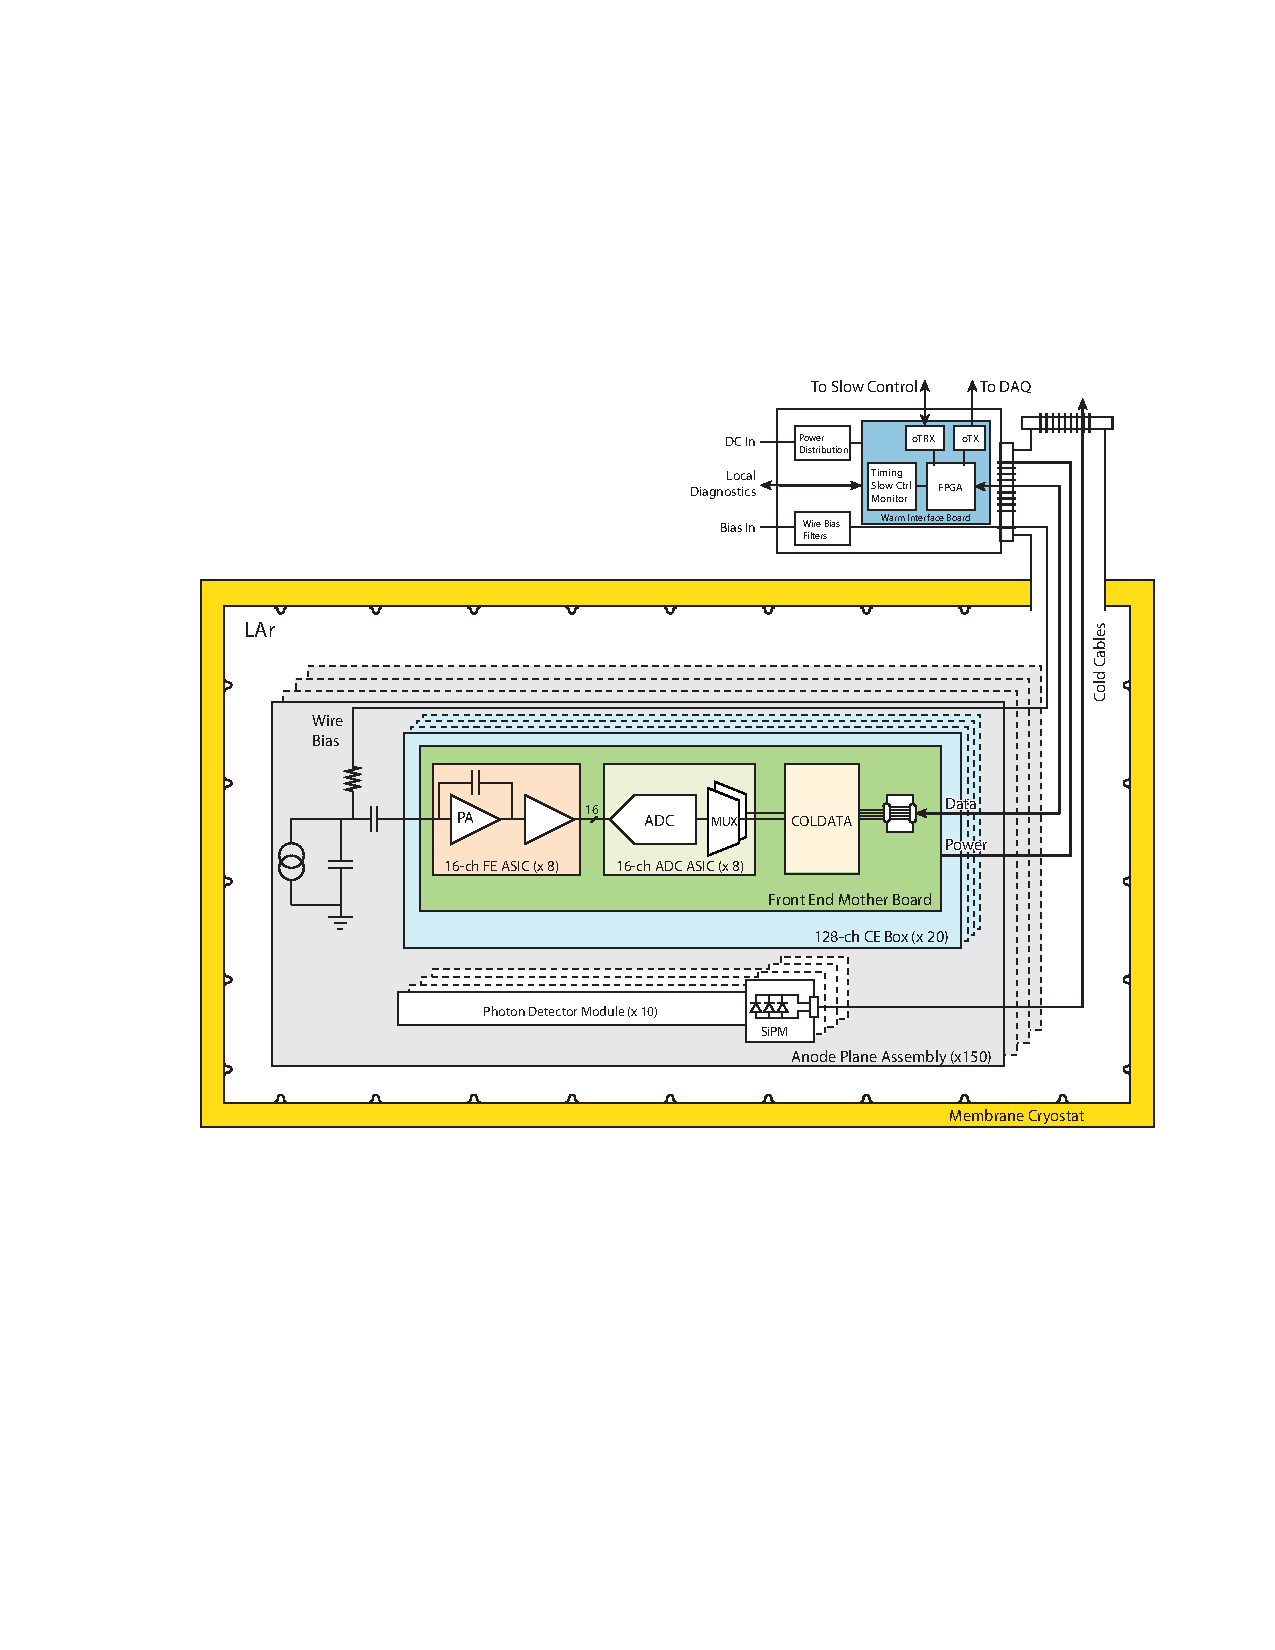
\includegraphics[width=0.85\textwidth]{Example_System_Level_Block-Diagram-SP_Cold_Electronics.pdf}
\end{dunefigure}


All consortia must provide an electrical wiring diagram which
represents the power and ground distribution within the system being
described.  The path of power and ground distribution wiring between
circuit elements are specified along with wire types and sizes.  Power
elements like power supplies, fuses (or other protective circuit
elements), power connectors and pin and wire ampacity are documented.


Electrical schematics show very specifically how individual
components are connected.  Usually, a schematic will represent a
printed circuit board design.  Schematics call out specific
parts that are used in the design and include all interconnections.
In the case of a printed circuit board, layout files, manufacturing
specifications, and bills of materials document
the design and allow a safety review of any custom boards or
modules.


Wiring diagrams include all wire and cable connections that run
between printed circuit boards or electronics modules.  Wires and
cables are described within the diagram and include identification of
American Wire Gauge \dword{awg}, wire color, cable specification and
cable connectors and pinouts.





\subsection{Electrical Integration Documentation}
\label{sec:fdsp-coord-integ-electrical}

Section~\ref{sec:fdsp-coord-electrical} listed the documentation
required to describe construction of a subsystem corresponding to the
design responsibilities within a consortium.  Interfaces that occur
between consortia subsystems must be documented and formally agreed
upon between the technical leads of the coordinating consortia and
must be verified by the \dword{tcoord} team.  Much of the
documentation required to describe a subsystem is also required for
integration.


Documentation required for the interface between two electrical
subsystems include a block diagram that identifies all connections
between the subsystems.  This block diagram must exist in the formal
interface document between consortia.  For each connection, additional
documentation must fully describe the interface
details. This additional detailed information can exist outside of the
primary interface document between consortia, but it must be pointed
to within that document.


One example of an integration interface is a signal cable that runs
between printed circuit boards belonging to different consortia.  For
a signal cable, interface documentation includes the connector
specifications, pinouts at each end of the cable and the pinout of the
board connectors.  Documentation also describes
relevant electrical signal characteristics that may include signal
levels, function, protocol, bandwidth and timing information.  If
signals are referred to using different signal names between
subsystems, documentation of signal name cross reference must be
provided.


Consortia technical leads and the \dword{tcoord} team must sign off
and approve the detailed documentation information on integration
interfaces not included in the primary consortia to consortia
interface document.

The \dword{tc} team will provide unique names and labels
for all racks, crates, boards, power supplies, cables and any other
electrical type equipment.  A database will be created to track these
devices.

\section{Configuration and Drawing Storage and Dissemination}
\label{sec:fdsp-coord-integ-modelplan}

The consortia and \dword{tc} engineering team create and share
drawings, models, schematics, production data and all other
engineering documents. In addition, the \dword{tc} engineering team
generates and shares all interface drawings and documentation.


Folders have been set up that allow uploading and sharing documents
with appropriate protection. The structure of the folders has been set
up to suit each consortium. The consortia do not necessarily have
similar folder structures or files and will adapt the structure to fit
their needs.


The folders and files reside on the \dword{edms}. This system and
similar structures were used for \dword{protodune} and are being
used by \dword{lbnf}.


The following shows a high-level outline of the file structure. The
first section is for technical coordination files. The second
section is generic, intended for a consortium. Each consortium will have one such
folder.
\begin{enumerate}
 \item Technical Coordination
 \begin{enumerate}
  \item Mechanical drawings and files (controlled by the lead mechanical engineer of \dword{dune})
  \begin{enumerate}
    \item Far Detector general drawings for illustration (controlled by \dword{tcoord})
    \item 3-D model files of internal detector for periodic upload to global model
    \item 2-D interface drawing files    
    \item Alignment and survey files
    \item Ash River installation test facility files
    \item \Dword{qa}/\dword{qc} files
    \item Safety analysis and documentation
    \item Design reviews
  \end{enumerate}
  \item Electrical and electronics (controlled by lead electrical engineer of \dword{dune})
  \begin{enumerate}
    \item Infrastructure requirements for grounding
    \item Consortia interface drawings
    \item Detector electronics grounding guidelines
    \item Detector safety system
    \item \dword{qa}/\dword{qc} files
    \item Safety analysis and documentation
  \end{enumerate}
 \end{enumerate}
 \item Consortia files (One per consortium, controlled by consortia technical leads)
 \begin{enumerate}
   \item 3-D Model files
   \item 2-D Part drawing files
   \item Production files
   \item General grounding diagrams
   \item System level block diagrams
   \item System level wiring diagrams
   \item Software and firmware plans
   \item Custom components, such as ASICs (one folder per component)
   \item PCB components (one folder per component)
   \item Cable components (one folder per component)
   \item Power supply components (one folder per component)
 \end{enumerate}
\end{enumerate}
(Note: add figure once the \dword{edms} structure is set up)


\section{ Organization of Interfaces and Interface Documents}
\label{sec:fdsp-coord-integ-interface}

To manage interfaces within the detector and between the detector and
facilities, an overall integration mechanism has been developed in
order to achieve an overall model.  The mechanism consisting of
defining integration nodes which can be thought of as focus areas as
explained below.  The interfaces between the nodes are carried out and
managed by the JPO engineering team.


\begin{dunefigure}[Integration Nodes.]{fig:integration_nodes}
  {Overall integration nodes and interfaces.}
  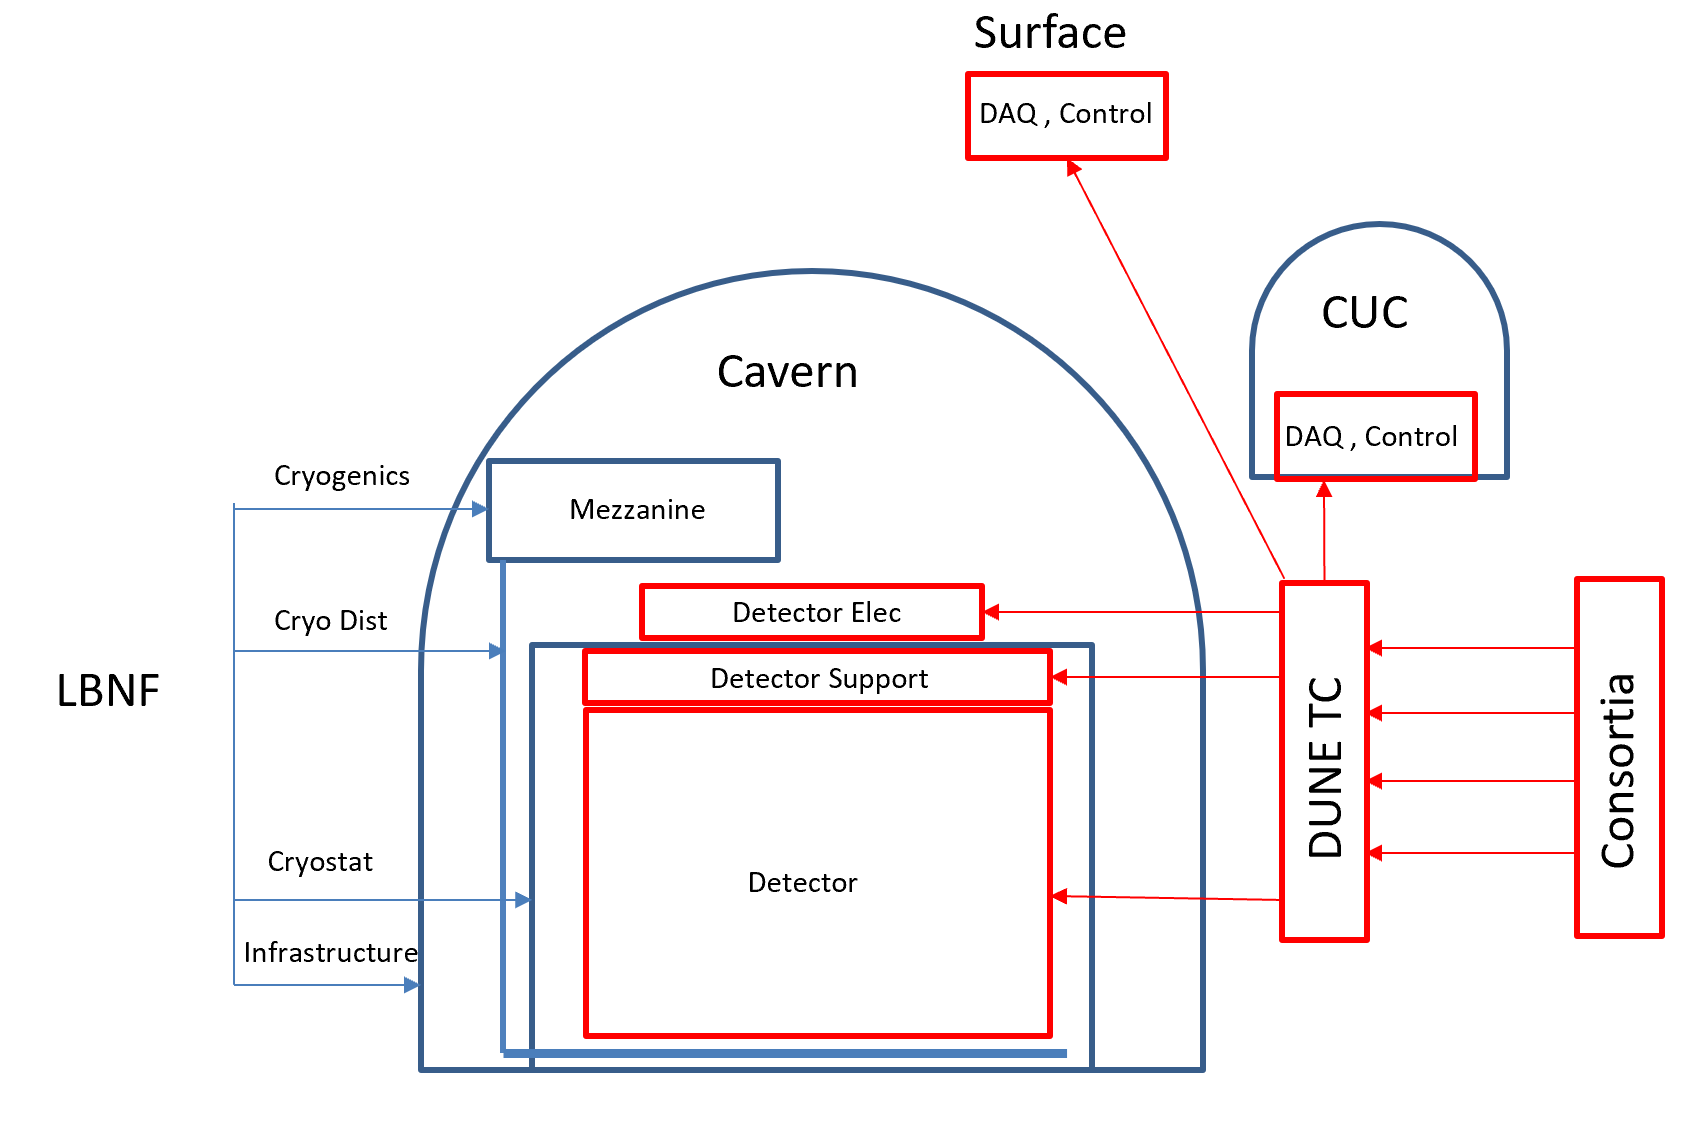
\includegraphics[width=0.7\textwidth]{Integration_nodes.png}
\end{dunefigure}

Figure~\ref{fig:integration_nodes} shows the interfaces between the
detector and facilities. In this figure, within the cavern, items
provided by \dword{lbnf} are on the left and the items provided by
\dword{dune} are on the right. In addition, the \dword{tc} engineering
team integrates the \dword{daq} room in the central utility cavern and
surface control and network rooms. Interfaces with \dword{lbnf} are
managed at the boundaries of each integration node. As an example, the
interface between \dword{lbnf} and \dword{dune} for the underground
\dword{daq} and control rooms are power, cooling water, data fibers
and cable penetrations at the room boundaries. Implementing power,
cooling water, data, and signal cables as well as integrating the
racks are the responsibilities of \dword{dune}.


The integration nodes comprise the following:
\begin{itemize}
\item {\bf Detector:} This consists of all \dword{tpc} elements within
  the \dword{lar}. Almost all consortia are involved in this
  integration task, which is mostly mechanical. Consortia engineering
  teams work directly with the \dword{tc} engineering team.  The
  primary interface is with \dword{dss} through hangers. Examples of
  interfaces within this node include: \dword{fc} connections to both
  \dwords{cpa} and \dwords{apa}, \dword{ce} and \dword{pd} cable
  routing within the cryostat and location of calibration and
  cryogenic instrumentation.
\item {\bf \dword{dss}:} This consists of all detector support elements,
  cable trays and feedthroughs.
\item {\bf Detector Electronics:} This consists of all racks, cooling,
  power, cable trays, cable distribution on top of cryostats, rack
  protection (smoke detectors, hardware power trip), rack component
  build and the interface to the \dword{ddss}.
\item {\bf \dword{daq} and Electronics:} This includes electronics on
  top of cryostat, in the \dword{daq} room and in the surface
  rooms. This also includes the fiber optic distribution from the
  surface to the \dword{daq} room and the fiber optic distribution
  from the detectors to the \dword{daq} room. It also includes the
  layout and cooling of the \dword{daq} room.
\end{itemize}

Interface documents are developed and maintained to manage the
interfaces among consortia and between consortia and \dword{tcoord}. A
single document covers the interface between any two systems, so any
one system may have several interface documents. If no interface
exists the interface document is not needed. The
interface documents are managed by relevant consortia technical leads
and by \dword{tc} project engineers.

The content of interface documents varies depending on the type
of interface. However, the documents are intended to have
a common structure, defining the interfaces in these sections:
\begin{enumerate}
 \item Definition: This section defines the interfacing systems.
 \item Hardware: In this section, the interfacing hardware components,
   electrical and mechanical, are defined in general terms. As an
   example, the \dword{apa} frame needs to support the \dword{pd}
   mounting brackets.
 \item Design: In this section, the dependencies in design
   methodology, sequence, and standards are described. As with the
   previous example, the design of the \dword{pd} mounting
   brackets depends on side tubes chosen for the \dword{apa}.
 \item Production: Component production and overall assembly is
   shared among interfacing systems. This section details who has what
   responsibilities.
 \item Testing: Like production, testing is a shared
   responsibility. In this section, responsibilities for testing and
   the required equipment are apportioned.
 \item Integration: The integration of systems into installable units
   before insertion into the cryostat is defined in this section. The
   location, methodology, tooling, and environment for integration are
   defined.
 \item Installation: Installation tasks and responsibilities, once
   installable units are assembled, are defined in this section. Any
   special transportation or installation tool or fixture is also
   defined.
 \item Commissioning: In this section, overall responsibilities for
   commissioning tasks are defined, and parameters are set.
 \item Appendices: Technical figures and interfaces should be included
   in this section in as much detail as necessary. Block diagrams that
   show interconnections and detailed documentation of each connection
   are needed.
\end{enumerate}

The interface documents will be developed and modified during the
technical design period. At the time of this writing, not all
documents have been fully developed. Once the technical design is
finished, the interface documents will be placed under revision
control.

\section{Enginering Change Control}
\label{sec:fdsp-change}

Changes in design and fabrication requirements follow revision process
for design and fabrication documents per consortia practice while
ensuring appropriate levels of verification, review and approval are
done by the consortia design authority.

Changes in design and fabrication requirements that involves
interfaces among consortia and between consortia and \dword{tc} may be
initiated and requested by consortia or \dword{tc}. Such changes are
handled by \dword{tc} through the Technical Board. Any change that
affect cost or schedule must involve Project Management.

When shop or site work must be performed before the affected design
document can be formally revised and re-issued such changes are
accomplished through the development, approval and distribution of an
Engineering Change Request (ECR). This process is for designs that are
under configuration management. Inter-discipline reviews shall be
performed when the ECR subject matter may impact other
disciplines. The design authority shall indicate if it is a one-time
change or if the change shall be incorporated into the design
documents.



\section{Value Engineering}
\label{sec:fdsp-coord-ve}

Value engineering is the process of arriving at cost effective
solutions to the technical challenges of building the \dword{dune}
detector. \dword{dune} value engineering builds on significant
developments in \dword{lar} detectors dating to the early 1970s,
especially the large \dwords{lartpc}: ICARUS and
\dword{microboone}. Prototyping by both LBNE and LBNO has
significantly advanced the value engineering process, leading to
construction of the \dword{protodune} detectors. These detectors validate
\dword{dune} designs and confirm that the necessary performance is
met. Any significant departure from current designs must account for
the success of \dword{protodune} and may require testing in a second
run of \dword{protodune}. 

The value engineering process is executed at both the consortia and
\dword{tc} level.For example, the \dword{apa} size has been optimized
over the last 10--15 years, using input from dimensions of the Ross
shaft, shipping container size and availability of high quality long
stainless steel tubes from reliable vendors.  At this point, any
significant change to the \dword{apa} design would likely lead to new
and significant re-engineering costs.

Value engineering is ongoing at all stages of design and will continue
through the fabrication, assembly and installation phases. In
particular, during fabrication and assembly stages, when labor costs
are relatively higher, it can result in significant cost savings. The
consortia and \dword{tc} are activley engaged and have the necessary
experience for this ongoing process.
